% !TeX root=SBUKThesis-main.tex
\clearpage
\thispagestyle{empty}

\chapter{پیشینه تحقیق و مفاهیم پایه}\label{chap2}

% فهرست مطالب فصل دوم
% \section*{فهرست مطالب}
% \begin{enumerate}
%     \item مقدمه
%     \item مفاهیم پایه
%     \begin{enumerate}
%         \item تکامل روش‌های یادگیری ماشین
%         \item انواع بدافزار (باج‌افزار، تروجان، جاسوس‌افزار، تبلیغ‌افزار)
%         \item مفاهیم مرتبط با اپلیکیشن‌های اندرویدی (مجوزها، فایل APK، سورس‌کد)
%         \item داده‌های چندوجهی در تشخیص بدافزار (جدولی، گرافی، ترتیبی)
%         \item مدل‌های یادگیری عمیق (CNN، RNN و LSTM، GNN، ترنسفورمر)
%         \item ماشین بردار پشتیبان (SVM)
%     \end{enumerate}
%     \item تکنیک‌های آموزشی و ارزیابی
%     \begin{enumerate}
%         \item اعتبارسنجی متقاطع (Cross-Validation)
%         \item مدیریت اورفیتینگ و آندرفیتینگ
%         \item روش‌های بهینه‌سازی (Adam, PIRATES, Optuna)
%         \item معیارهای ارزیابی عملکرد (Accuracy, F1 Score, AUC)
%     \end{enumerate}
%     \item مروری بر مطالعات پیشین
%     \begin{enumerate}
%         \item روش‌های تحلیل ایستا
%         \item روش‌های تحلیل پویا
%         \item کارهای پیشین و تاریخچه مختصر
%     \end{enumerate}
%     \item جمع‌بندی فصل
% \end{enumerate}

\section{مقدمه}
در سال‌های اخیر، با گسترش روزافزون استفاده از دستگاه‌های هوشمند مبتنی بر سیستم‌عامل اندروید، امنیت سایبری به یکی از دغدغه‌های اصلی کاربران و سازمان‌ها تبدیل شده است. محبوبیت گسترده اندروید، که طبق آمار \lr{Statista} در سال ۲۰۲۴ بیش از ۷۰ درصد بازار جهانی دستگاه‌های هوشمند را در اختیار دارد \cite{Statista2024}، آن را به هدف اصلی حملات بدافزاری، از جمله تروجان‌ها\LTRfootnote{Trojan}، جاسوس‌افزارها\LTRfootnote{Spyware} و باج‌افزارها\LTRfootnote{Ransomware}، مبدل ساخته است \cite{AndroidSecurity}. این تهدیدات، با بهره‌گیری از روش‌های پیچیده و نوظهور، چالش‌های جدی در شناسایی و خنثی‌سازی ایجاد کرده‌اند، به‌ویژه در مورد بدافزارهای ناشناخته (Zero-Day)\LTRfootnote{Zero-Day} که تشخیص آن‌ها با روش‌های سنتی مبتنی بر امضا دشوار است \cite{AndroidMalwareSurvey}. از این رو، توسعه مدل‌های پیشرفته مبتنی بر یادگیری عمیق و داده‌های چندوجهی، به‌عنوان راهکاری نوین برای مقابله با این تهدیدات، مورد توجه فزاینده‌ای قرار گرفته است \cite{DeepLearningMalware}.

فصل حاضر به‌عنوان پایه‌ای برای درک روش پیشنهادی این پژوهش، به بررسی مفاهیم پایه و مرور مطالعات پیشین در حوزه تشخیص بدافزارهای اندرویدی می‌پردازد. ابتدا، مفاهیم کلیدی و اصطلاحات فنی مورد نیاز معرفی خواهند شد. سپس، تکنیک‌های رایج یادگیری ماشین و یادگیری عمیق که در این حوزه کاربرد دارند، تشریح می‌شوند. در ادامه، ابزارها و روش‌های بهینه‌سازی مانند ترنسفورمرها\LTRfootnote{Transformer}، الگوریتم‌های \lr{PIRATES} و \lr{Optuna}\LTRfootnote{Optuna}، که در طراحی مدل \lr{MAGNET} (روش پیشنهادی این پژوهش) به کار رفته‌اند، معرفی خواهند شد. همچنین، تکنیک‌های آموزشی و معیارهای ارزیابی عملکرد، نظیر اعتبارسنجی متقاطع\LTRfootnote{Cross-Validation} و معیارهای دقت\LTRfootnote{Accuracy}، \lr{F1 Score}\LTRfootnote
 و \lr{AUC}\LTRfootnote{Area Under Curve (AUC)}، به‌منظور تبیین چارچوب ارزیابی مدل توضیح داده می‌شوند.

در بخش بعدی، پیشینه تحقیق با تمرکز بر روش‌های تحلیل ایستا\LTRfootnote{Static Analysis} و پویا\LTRfootnote{Dynamic Analysis}، که پایه‌های اصلی تشخیص بدافزار را تشکیل می‌دهند، مورد بررسی قرار می‌گیرد. این مرور، با تحلیل نقاط قوت و ضعف روش‌های پیشین، زمینه‌ای برای درک نوآوری‌های مدل پیشنهادی فراهم می‌کند. هدف این فصل، ارائه دیدگاهی جامع و منسجم از مفاهیم و مطالعات مرتبط است تا خواننده را برای درک بهتر روش‌شناسی و نتایج پژوهش آماده سازد. این ساختار، نه‌تنها به تبیین مسائل نظری کمک می‌کند، بلکه راه را برای مقایسه و ارزیابی عملکرد مدل \lr{MAGNET} هموار می‌سازد.

\section{مفاهیم پایه}
در این بخش، مفاهیم بنیادی مرتبط با موضوع پژوهش، از جمله تاریخچه مختصری از یادگیری ماشین، انواع بدافزارها، ساختار اپلیکیشن‌های اندروید، داده‌های چندوجهی و مدل‌های یادگیری عمیق مرتبط، تشریح می‌شوند.

\subsection{تکامل روش‌های یادگیری ماشین}
در دهه‌های ۱۹۵۰ و ۱۹۶۰، اولین تلاش‌ها برای پردازش زبان طبیعی به وسیله‌ی روش‌های نمادین انجام شد. پژوهشگران در آن زمان سعی می‌کردند ساختارهای دستوری و قوانین زبان را به صورت صریح و دستی تعریف کنند. این رویکردها با وجود تلاش‌های ارزشمند، به دلیل محدودیت‌های محاسباتی و عدم وجود داده‌های کافی، نتوانستند به دقت و کارایی مورد انتظار دست یابند.

با گذر زمان و ورود به دهه‌های ۱۹۶۰ و ۱۹۷۰، رویکردهای آماری جایگزین بخش‌هایی از روش‌های نمادین شدند. در این دوران، مدل‌های \lr{n-gram} که بر مبنای احتمال وقوع یک کلمه با توجه به کلمات قبلی محاسبه می‌شدند، به عنوان اولین قدم‌های موفق در مدلسازی زبان مطرح شدند. اگرچه این مدل‌ها ساده بودند، اما توانستند برخی از پیچیدگی‌های اولیه‌ی پردازش زبان را کاهش دهند.

در دهه‌های ۱۹۸۰ و ۱۹۹۰، با پیشرفت‌های چشمگیر در فناوری‌های محاسباتی و افزایش دسترسی به داده‌های متنی، روش‌های یادگیری ماشین وارد عرصه شدند. الگوریتم‌های یادگیری نظارت‌شده و غیرنظارتی به منظور تشخیص الگوهای زبانی به کار گرفته شدند. با این حال، محدودیت‌های موجود همچنان مانع از دستیابی به درک عمیق‌تر و تولید متن‌های طبیعی به سطح امروزی می‌شدند.

ورود به قرن ۲۱ و به‌ویژه دهه ۲۰۱۰، با ظهور شبکه‌های عصبی عمیق مانند شبکه‌های عصبی کانولوشنی
\LTRfootnote{Convolutional Neural Networks (CNNs)}
، شبکه‌های عصبی بازگشتی
\LTRfootnote{Recursive Neural Networks (RNNs)}
 و شبکه‌های حافظه بلندمدت-کوتاه‌مدت
\LTRfootnote{Long Short-Term Memory (LSTM)}
  همراه بود. این مدل‌ها توانستند وابستگی‌های زمانی، الگوهای تصویری و روابط بلندمدت موجود در داده‌ها را بهتر مدل‌سازی کنند \cite{Vinayakumar2019}. با این حال، چالش‌هایی همچنان در زمینه بهبود کیفیت و کارایی تحلیل داده‌های پیچیده مانند کدهای بدافزار وجود داشت که منجر به توسعه معماری‌های پیشرفته‌تری مانند ترنسفورمرها شد.

\subsection{انواع بدافزار}
بدافزار (Malware) اصطلاحی کلی برای هر نوع نرم‌افزار مخرب است که با هدف آسیب رساندن به سیستم‌ها، سرقت اطلاعات یا اختلال در عملکرد طراحی می‌شود. در ادامه، برخی از رایج‌ترین انواع بدافزارها معرفی می‌شوند:

\subsubsection{باج‌افزار}
باج‌افزار\LTRfootnote{Ransomware} گونه‌ای از بدافزارها است که با سرعت زیادی گسترش یافته و امروزه به شکل فراگیری در حال شیوع است. باج‌افزارها عمدتاً به دو نوع قفل‌کننده (کریپتور)\LTRfootnote{Cryptor} و مسدودکننده\LTRfootnote{Locker} تقسیم می‌شوند. پس از آلوده‌سازی رایانه، نوع قفل‌کننده داده‌های ارزشمند کاربر از جمله اسناد، تصاویر و پایگاه‌های داده را رمزنگاری می‌کند و تا زمانی که رمزگشایی نشوند، هیچ فایلی قابل دسترسی نخواهد بود. مهاجمان در ازای ارائه کلید رمزگشا برای بازگرداندن فایل‌های قفل‌شده، درخواست باج می‌کنند. نوع مسدودکننده نیز دسترسی به کل سیستم آلوده را مسدود می‌کند و معمولاً میزان باج‌خواهی آن کمتر از نوع قفل‌کننده است.

باج‌افزارها می‌توانند سیستم‌عامل‌های مختلفی مانند ویندوز، مک‌اواس\LTRfootnote{Mac OS X}، لینوکس و اندروید را هدف قرار دهند و هم رایانه‌های دسکتاپ و هم دستگاه‌های موبایل را آلوده سازند \cite{AndroidSecurity}. آلودگی معمولاً از طریق باز کردن فایل‌های ضمیمه مخرب، کلیک روی لینک‌های مشکوک یا نصب برنامه‌ها از منابع غیررسمی رخ می‌دهد. حتی وب‌سایت‌های رسمی نیز گاهی به واسطه شبکه‌های تبلیغاتی آلوده می‌شوند. حذف باج‌افزارها معمولاً دشوار است و در صورت رمزنگاری فایل‌ها، کاربر باید برای بازیابی دسترسی، رمزگشایی انجام دهد که پرداخت باج نیز تضمینی برای بازگشت اطلاعات نیست و توصیه نمی‌شود.

\subsubsection{تروجان}
تروجان\LTRfootnote{Trojan Horse} یا اسب تروآ، نوعی برنامه مخرب است که خود را به عنوان نرم‌افزاری مشروع و بی‌خطر جلوه می‌دهد تا کاربر را فریب داده و به سیستم نفوذ کند. نام‌گذاری این بدافزار برگرفته از داستان اسب چوبی تروای یونانیان است که با حیله وارد شهر شد. انواع مختلفی از تروجان‌ها وجود دارد، از جمله:
\begin{itemize}
    \item \textbf{تروجان دسترسی از راه دور \lr{(Backdoor)}:} به مهاجم امکان کنترل سیستم قربانی از راه دور را می‌دهد.
    \item \textbf{تروجان ارسال داده:} اطلاعات حساس مانند رمزهای عبور و داده‌های واردشده توسط کاربر را به مهاجم ارسال می‌کند.
    \item \textbf{تروجان مخرب:} فایل‌های سیستمی را حذف یا تخریب می‌کند.
    \item \textbf{تروجان \lr{DoS}:} باعث کاهش سرعت سیستم و اینترنت کاربر می‌شود (حملات منع سرویس).
    \item \textbf{تروجان پراکسی:} به مهاجم اجازه می‌دهد از طریق سیستم قربانی به سرورهای پراکسی حمله کند.
    \item \textbf{تروجان \lr{FTP}:} پورت \lr{FTP} را باز کرده و کنترل سیستم را از این طریق به مهاجم می‌دهد.
    \item \textbf{تروجان غیرفعال‌سازی امنیت:} نرم‌افزارهای امنیتی را غیرفعال می‌کند تا حمله آسان‌تر انجام شود.
\end{itemize}

\subsubsection{جاسوس‌افزار}
جاسوس‌افزار\LTRfootnote{Spyware} نوعی نرم‌افزار مخرب است که بدون اطلاع کاربر، اطلاعاتی درباره او یا فعالیت‌هایش را جمع‌آوری و برای مهاجم ارسال می‌کند. کاربردهای رایج جاسوس‌افزارها شامل تبلیغات هدفمند، جمع‌آوری اطلاعات شخصی (مانند اطلاعات بانکی یا رمزهای عبور) و ایجاد تغییرات ناخواسته در تنظیمات سیستم قربانی است. این بدافزارها می‌توانند باعث کاهش کارایی سیستم، نصب نوارابزارهای ناخواسته، تغییر صفحه خانگی مرورگر و باز شدن صفحات پاپ‌آپ تبلیغاتی شوند.

\subsubsection{تبلیغ‌افزار}
تبلیغ‌افزار\LTRfootnote{Adware} نرم‌افزاری است که با هدف نمایش تبلیغات ناخواسته روی سیستم قربانی طراحی شده است. این تبلیغات معمولاً به صورت بنرها یا صفحات پاپ‌آپ ظاهر می‌شوند و گاهی صفحات اینترنتی متعددی را به طور متوالی باز می‌کنند. اگرچه همه تبلیغ‌افزارها ذاتاً مخرب نیستند (برخی نرم‌افزارهای رایگان از طریق نمایش تبلیغ درآمدزایی می‌کنند)، اما انواع تهاجمی آن‌ها می‌توانند فعالیت‌های آنلاین کاربر را دنبال کرده و تجربه کاربری را مختل کنند. همچنین، برخی تبلیغ‌افزارها اطلاعات مربوط به رفتار کاربر را جمع‌آوری و برای اهداف تبلیغاتی یا حتی فروش به اشخاص ثالث ارسال می‌کنند که می‌تواند حریم خصوصی را نقض کند.

\subsection{مفاهیم مرتبط با اپلیکیشن‌های اندرویدی}

\subsubsection{مجوزهای دسترسی}
اندروید از یک سیستم تخصیص مجوز\LTRfootnote{Permission System} برخوردار است که برای هر عملیات یا وظیفه (\lr{Task}) حساس، مجوزها و سطوح دسترسی خاصی را تعیین می‌کند. هر اپلیکیشن می‌تواند برای انجام عملیات خاص، مجوزهای لازم را از این سامانه درخواست نماید. به عنوان مثال، یک برنامه کاربردی ممکن است برای دسترسی به اینترنت، دوربین، یا لیست مخاطبین، مجوزهای مربوطه را درخواست کند. این سیستم دارای سطوح مختلفی برای مجوزها است که به آن‌ها سطح حفاظت (\lr{Protection Level}) گفته می‌شود.

در نسخه‌های قدیمی‌تر اندروید (قبل از نسخه ۶.۰)، اپلیکیشن‌ها هنگام نصب، لیست تمامی مجوزهای مورد نیاز خود را به کاربر اعلام می‌کردند و کاربر یا همه را می‌پذیرفت یا نصب را لغو می‌کرد. اما از نسخه ۶.۰ اندروید (\lr{Marshmallow}، \lr{API} سطح ۲۳) به بعد، مدل مجوزدهی پویا (\lr{Runtime Permissions}) معرفی شد که طی آن، مجوزهای حساس تنها در زمان اجرای برنامه و هنگامی که اپلیکیشن برای اولین بار به آن قابلیت نیاز دارد، از کاربر درخواست می‌شوند. اپلیکیشن‌های اندرویدی مجوزهای مورد نیاز خود را در فایل مانیفست اندروید (\lr{AndroidManifest.xml}) اعلام می‌کنند. همچنین، اپلیکیشن می‌تواند مجوزهای اضافی را در این فایل تعریف کند که دسترسی به برخی اجزای داخلی نرم‌افزار توسط سایر برنامه‌ها را محدود می‌سازد.

در اندروید، مجوزها عمدتاً به دو سطح دسترسی و امنیت تقسیم می‌شوند:
\begin{itemize}
    \item \textbf{معمولی \lr{(Normal)}:} مجوزهایی که ریسک پایینی برای حریم خصوصی کاربر یا عملکرد سایر اپلیکیشن‌ها دارند (مانند مجوز دسترسی به اینترنت یا تنظیم منطقه زمانی). این مجوزها معمولاً به صورت خودکار هنگام نصب یا به‌روزرسانی به اپلیکیشن اعطا می‌شوند و نیازی به تأیید صریح کاربر ندارند.
    \item \textbf{خطرناک \lr{(Dangerous)}:} مجوزهایی که به اطلاعات خصوصی کاربر (مانند مخاطبین، موقعیت مکانی، پیامک‌ها) دسترسی دارند یا می‌توانند بر عملکرد دستگاه یا سایر اپلیکیشن‌ها تأثیر بگذارند (مانند دسترسی به دوربین یا میکروفون). این مجوزها باید حتماً در زمان اجرا و به صورت صریح از کاربر درخواست شوند.
\end{itemize}
تحلیل الگوهای درخواست مجوز یکی از روش‌های مهم در تشخیص بدافزارهای اندرویدی است، زیرا بدافزارها اغلب مجوزهای خطرناک بیشتری نسبت به کاربرد ظاهری خود درخواست می‌کنند \cite{Drebin}.

\subsubsection{فایل APK}
فرمت \lr{APK}\LTRfootnote{Android Package Kit} مخفف عبارت \lr{Android Package Kit} است و فرمت فایل بسته‌بندی شده‌ای است که برای توزیع و نصب برنامه‌ها و میان‌افزارها در سیستم‌عامل اندروید استفاده می‌شود. فایل \lr{APK} شامل تمام کدهای برنامه (مانند فایل‌های \lr{.dex})، منابع (مانند تصاویر و لایه‌ها)، دارایی‌ها، گواهی‌نامه‌ها و فایل مانیفست (\lr{AndroidManifest.xml}) است. این فایل بسیار شبیه به فرمت‌های بسته‌بندی دیگر مانند \lr{APPX} در مایکروسافت ویندوز یا \lr{.deb} در سیستم‌های مبتنی بر دبیان (مانند اوبونتو) عمل می‌کند.

برای ساخت یک فایل \lr{APK}، ابتدا برنامه اندروید با استفاده از ابزارهایی مانند اندروید استودیو کامپایل شده و سپس تمام اجزای آن در یک فایل فشرده با پسوند \lr{.apk} بسته‌بندی می‌شود. فایل‌های \lr{APK} پایه و اساس برنامه‌های اندرویدی هستند و بخش اصلی اکوسیستم اندروید محسوب می‌شوند. کاربران می‌توانند فایل‌های \lr{APK} را از منابع مختلف، از جمله فروشگاه رسمی گوگل پلی (\lr{Google Play}) یا به صورت دستی (Sideloading) از وب‌سایت‌ها یا منابع دیگر، دانلود و نصب کنند. نصب دستی برنامه‌ها از منابع نامعتبر یکی از راه‌های اصلی ورود بدافزار به دستگاه‌های اندرویدی است.

علاوه بر سیستم‌عامل اندروید، فایل‌های \lr{APK} را می‌توان با استفاده از شبیه‌سازها یا لایه‌های سازگاری در سایر سیستم‌عامل‌ها مانند ویندوز، مک‌اواس یا کروم‌اواس نیز اجرا، و با ابزارهای مهندسی معکوس، محتوای آن‌ها را استخراج، ویرایش یا تحلیل کرد.

\subsubsection{سورس‌کد}
سورس‌کد (\lr{Source Code}) یا کد منبع برنامه، به مجموعه‌ای از دستورالعمل‌ها یا عبارات متنی اشاره دارد که توسط برنامه‌نویس به یک زبان برنامه‌نویسی خاص (مانند جاوا، کاتلین، \lr{++C}، پایتون) نوشته می‌شود تا یک برنامه کامپیوتری، عملکرد مورد نظر را پیاده‌سازی کند. سورس‌کد برای انسان قابل خواندن است و منطق، الگوریتم‌ها و ساختار برنامه را تعریف می‌کند.

برای اینکه کامپیوتر بتواند سورس‌کد را اجرا کند، باید ابتدا به زبان ماشین (کد باینری) ترجمه شود. این فرآیند توسط یک کامپایلر یا مفسر انجام می‌شود. در اکوسیستم اندروید، کدهای جاوا یا کاتلین معمولاً به بایت‌کد \lr{Dalvik} (در نسخه‌های قدیمی‌تر) یا \lr{ART} \lr{(Android Runtime)} کامپایل می‌شوند که در فایل‌های \lr{.dex} درون فایل \lr{APK} قرار می‌گیرند.

دسترسی به سورس‌کد یک برنامه امکان درک کامل عملکرد، اصلاح یا توسعه آن را فراهم می‌کند. در حوزه امنیت، تحلیل سورس‌کد (در صورت در دسترس بودن) یکی از روش‌های تحلیل ایستا برای یافتن آسیب‌پذیری‌ها یا کدهای مخرب است. با این حال، اکثر برنامه‌های تجاری یا بدافزارها به صورت کامپایل‌شده و بدون سورس‌کد توزیع می‌شوند و تحلیل آن‌ها نیازمند مهندسی معکوس (مانند دیس‌اسمبل کردن کدهای باینری یا بایت‌کد) است.

\subsection{داده‌های چندوجهی در تشخیص بدافزار}
داده‌های چندوجهی (\lr{Multi-Modal Data}) به مجموعه‌ای از اطلاعات اشاره دارد که از منابع و قالب‌های متنوعی استخراج شده و برای تحلیل جامع‌تر یک پدیده، مانند تشخیص بدافزارهای اندرویدی، به کار می‌روند. در این پژوهش، مدل \lr{MAGNET} با بهره‌گیری از سه نوع اصلی داده‌های چندوجهی، شامل داده‌های جدولی، گرافی و ترتیبی، طراحی شده است تا بتواند ویژگی‌های متنوع و مکمل اپلیکیشن‌های اندرویدی را به‌صورت یکپارچه پردازش کند. این رویکرد، برخلاف روش‌های سنتی که تنها به یک نوع داده (مثلاً فقط مجوزها یا فقط فراخوانی‌های \lr{API}) وابسته‌اند، امکان درک عمیق‌تر رفتارهای مخرب را فراهم می‌سازد. در ادامه، هر یک از این انواع داده‌ها به‌طور جداگانه توضیح داده می‌شود.

\subsubsection{داده‌های جدولی}
داده‌های جدولی شامل ویژگی‌های ایستای اپلیکیشن‌های اندرویدی هستند که به‌صورت ساختارمند و معمولاً عددی یا دسته‌ای ارائه می‌شوند. این ویژگی‌ها می‌توانند شامل تعداد مجوزهای درخواست‌شده، اندازه فایل \lr{APK}، نسخه \lr{SDK} هدف، تعداد فعالیت‌ها (\lr{Activities})، سرویس‌ها (\lr{Services})، گیرنده‌های پخش (\lr{Broadcast Receivers})، ارائه‌دهندگان محتوا (\lr{Content Providers})، تعداد فراخوانی‌های \lr{API} خاص، یا سایر متغیرهای استخراج‌شده از فایل \lr{AndroidManifest.xml} یا کد کامپایل شده باشند. در این پژوهش، این داده‌ها با استفاده از کتابخانه \lr{PyTorch} و به‌صورت اشیای تانسور (\lr{torch.Tensor}) بارگذاری و پردازش می‌شوند. برای هر نمونه اپلیکیشن، یک بردار ویژگی با ابعاد مشخص تعریف می‌شود که نشان‌دهنده خصوصیات ایستای آن است. پیش‌پردازش این داده‌ها، مانند نرمال‌سازی (برای مقادیر عددی) یا کدگذاری وان‌هات (برای مقادیر دسته‌ای)، که با هدف بهبود عملکرد مدل انجام می‌شود، از مراحل کلیدی به شمار می‌رود. این نوع داده، پایه‌ای برای تحلیل‌های آماری و یادگیری الگوهای ساده در بدافزارها فراهم می‌کند (مثلاً بدافزارها ممکن است به طور متوسط مجوزهای بیشتری درخواست کنند).

\subsubsection{داده‌های گرافی}
داده‌های گرافی ساختارهایی هستند که روابط و تعاملات بین اجزای مختلف یک اپلیکیشن اندرویدی را مدل‌سازی می‌کنند. این داده‌ها می‌توانند نمایانگر گراف فراخوانی توابع (\lr{Call Graph})، گراف جریان کنترل (\lr{Control Flow Graph, CFG})، گراف وابستگی داده‌ها (\lr{Data Dependency Graph})، یا گراف روابط بین اجزای برنامه (مانند ارتباط بین فعالیت‌ها از طریق \lr{Intents}) باشند. گره‌ها (\lr{Nodes}) در این گراف‌ها می‌توانند توابع، بلوک‌های کد، کلاس‌ها، مجوزها یا اجزای اندرویدی باشند و لبه‌ها (\lr{Edges}) نشان‌دهنده روابطی مانند فراخوانی تابع، انتقال کنترل، جریان داده یا درخواست مجوز هستند. در این پژوهش، از کتابخانه \lr{PyTorch Geometric} (\lr{torch\_geometric}) برای بارگذاری و پردازش این داده‌ها به‌صورت اشیای داده (\lr{Data}) استفاده شده است. هر گراف شامل ماتریس همجواری (ساختار گراف) و ویژگی‌های گره‌ها (مانند نوع تابع یا بردار ویژگی‌های استخراج‌شده از کد) است. تحلیل گرافی به مدل اجازه می‌دهد تا الگوهای ساختاری پیچیده و وابستگی‌های پنهان بین اجزا را شناسایی کند (مانند شناسایی یک حلقه فراخوانی مشکوک یا یک خوشه از توابع مرتبط با سرقت اطلاعات)، که در تشخیص بدافزارهای پیچیده یا ناشناخته بسیار مؤثر است.

\subsubsection{داده‌های ترتیبی}
داده‌های ترتیبی شامل توالی‌هایی از رویدادها یا مقادیر هستند که معمولاً نمایانگر رفتار زمانی یا ترتیب وقوع عملیات در اپلیکیشن‌ها هستند. در زمینه تشخیص بدافزار اندروید، این داده‌ها می‌توانند شامل توالی فراخوانی‌های \lr{API} سیستمی در حین اجرای برنامه (استخراج‌شده از تحلیل پویا)، توالی رویدادهای سیستمی (مانند ارسال پیامک، اتصال به شبکه)، یا الگوهای زمانی استفاده از منابع (مانند مصرف \lr{CPU} یا باتری) باشند. در این پژوهش، این داده‌ها با استفاده از تانسورهای \lr{LongTensor} در \lr{PyTorch} بارگذاری شده و برای هر نمونه یک یا چند توالی مشخص تعریف می‌شود. پیش‌پردازش این داده‌ها ممکن است شامل نگاشت هر رویداد یا \lr{API} به یک شناسه عددی، پدینگ (\lr{Padding}) توالی‌ها برای رسیدن به طول یکسان، و تبدیل به فرمت قابل پردازش توسط مدل‌های ترتیبی مانند \lr{RNN}، \lr{LSTM} یا ترنسفورمر باشد. استفاده از داده‌های ترتیبی به مدل امکان می‌دهد تا رفتار پویای اپلیکیشن‌ها را تحلیل کند و الگوهای زمانی مخرب، مانند توالی خاصی از فراخوانی‌ها که منجر به نشت داده می‌شود یا حملات دوره‌ای، را تشخیص دهد.

\subsubsection{اهمیت و یکپارچگی داده‌های چندوجهی}
ترکیب این سه نوع داده در مدل \lr{MAGNET}، با استفاده از مکانیزم‌های توجه پویا و تکنیک‌های همجوشی (\lr{Fusion})، به شناسایی دقیق‌تر و جامع‌تر بدافزارها کمک می‌کند. داده‌های جدولی اطلاعات کلی و ایستا، داده‌های گرافی روابط ساختاری پیچیده، و داده‌های ترتیبی رفتار پویا را ارائه می‌دهند که در کنار هم، تصویری کامل‌تر از اپلیکیشن را ترسیم می‌کنند. این رویکرد چندوجهی، به‌ویژه در مواجهه با بدافزارهای پیچیده و ناشناخته که ممکن است در یک وجه خاص (مثلاً فقط مجوزها) عادی به نظر برسند، مزیت رقابتی نسبت به روش‌های تک‌وجهی دارد و تعمیم‌پذیری مدل را افزایش می‌دهد \cite{Marastoni2022}. استخراج این داده‌ها از فایل‌های پردازش‌شده با توابع فرضی \lr{load\_processed\_data}، \lr{load\_graph\_data}، و \lr{load\_sequence\_data} انجام شده و پیش‌پردازش آن‌ها با نرمال‌سازی، استانداردسازی و کدگذاری مناسب، تضمین‌کننده سازگاری با معماری‌های یادگیری عمیق مانند ترنسفورمر است.

\subsection{مدل‌های یادگیری عمیق}
یادگیری عمیق، زیرشاخه‌ای از یادگیری ماشین، از شبکه‌های عصبی مصنوعی با چندین لایه (لایه‌های عمیق) برای یادگیری بازنمایی‌های پیچیده از داده‌ها استفاده می‌کند. در ادامه، چند معماری کلیدی که در تشخیص بدافزار کاربرد دارند، معرفی می‌شوند.

\subsubsection{شبکه‌های عصبی کانولوشنی (CNN)}
شبکه‌های عصبی کانولوشنی (\lr{Convolutional Neural Networks, CNNs}) به طور خاص برای پردازش داده‌های با ساختار شبکه‌ای یا گریدمانند، مانند تصاویر، ماتریس‌های ویژگی یا داده‌های ترتیبی با پنجره لغزان، طراحی شده‌اند. این شبکه‌ها با بهره‌گیری از لایه‌های کانولوشنی که فیلترهای کوچکی را روی ورودی حرکت می‌دهند، قادرند ویژگی‌های محلی (مانند الگوهای خاص در بایت‌های کد، توالی‌های \lr{API}، یا روابط بین مجوزها در یک ماتریس هم‌وقوعی) را به صورت سلسله‌مراتبی و خودکار استخراج کنند. لایه‌های تجمعی (\lr{Pooling}) نیز با کاهش ابعاد مکانی داده و فشرده‌سازی اطلاعات، به افزایش پایداری نسبت به تغییرات جزئی و کاهش محاسبات کمک می‌کنند. در نهایت، لایه‌های کاملاً متصل (\lr{Fully Connected}) از ویژگی‌های استخراج‌شده برای طبقه‌بندی نهایی (مثلاً بدافزار یا سالم) استفاده می‌کنند. در حوزه تشخیص بدافزار، شبکه‌های \lr{CNN} می‌توانند برای تحلیل بایت‌های فایل اجرایی به عنوان تصویر \cite{Nataraj2011}، ماتریس‌های ویژگی‌های ایستا، یا توالی‌های رفتاری به کار روند و الگوهای مخرب را شناسایی نمایند \cite{Vinayakumar2019}.

تحقیقات اخیر نشان داده است که شبکه‌های عصبی کانولوشنی می‌توانند دقت بالایی در تشخیص بدافزار ارائه دهند و ویژگی‌های مورد نیاز را مستقیماً از داده‌های خام یا نیمه‌پردازش‌شده یاد بگیرند \cite{Alsaleh2023}. ساختار این شبکه‌ها معمولاً به صورت انتها به انتها (\lr{End-to-End}) طراحی می‌شود و شامل پشته‌ای از لایه‌های کانولوشنی، فعال‌سازی (مانند \lr{ReLU})، و تجمعی است که به دنبال آن یک یا چند لایه کاملاً متصل قرار می‌گیرد. افزایش عمق شبکه (تعداد لایه‌ها) امکان استخراج ویژگی‌های انتزاعی‌تر و سطح بالاتر را فراهم می‌کند.

\begin{figure}[!t]
    \centering
    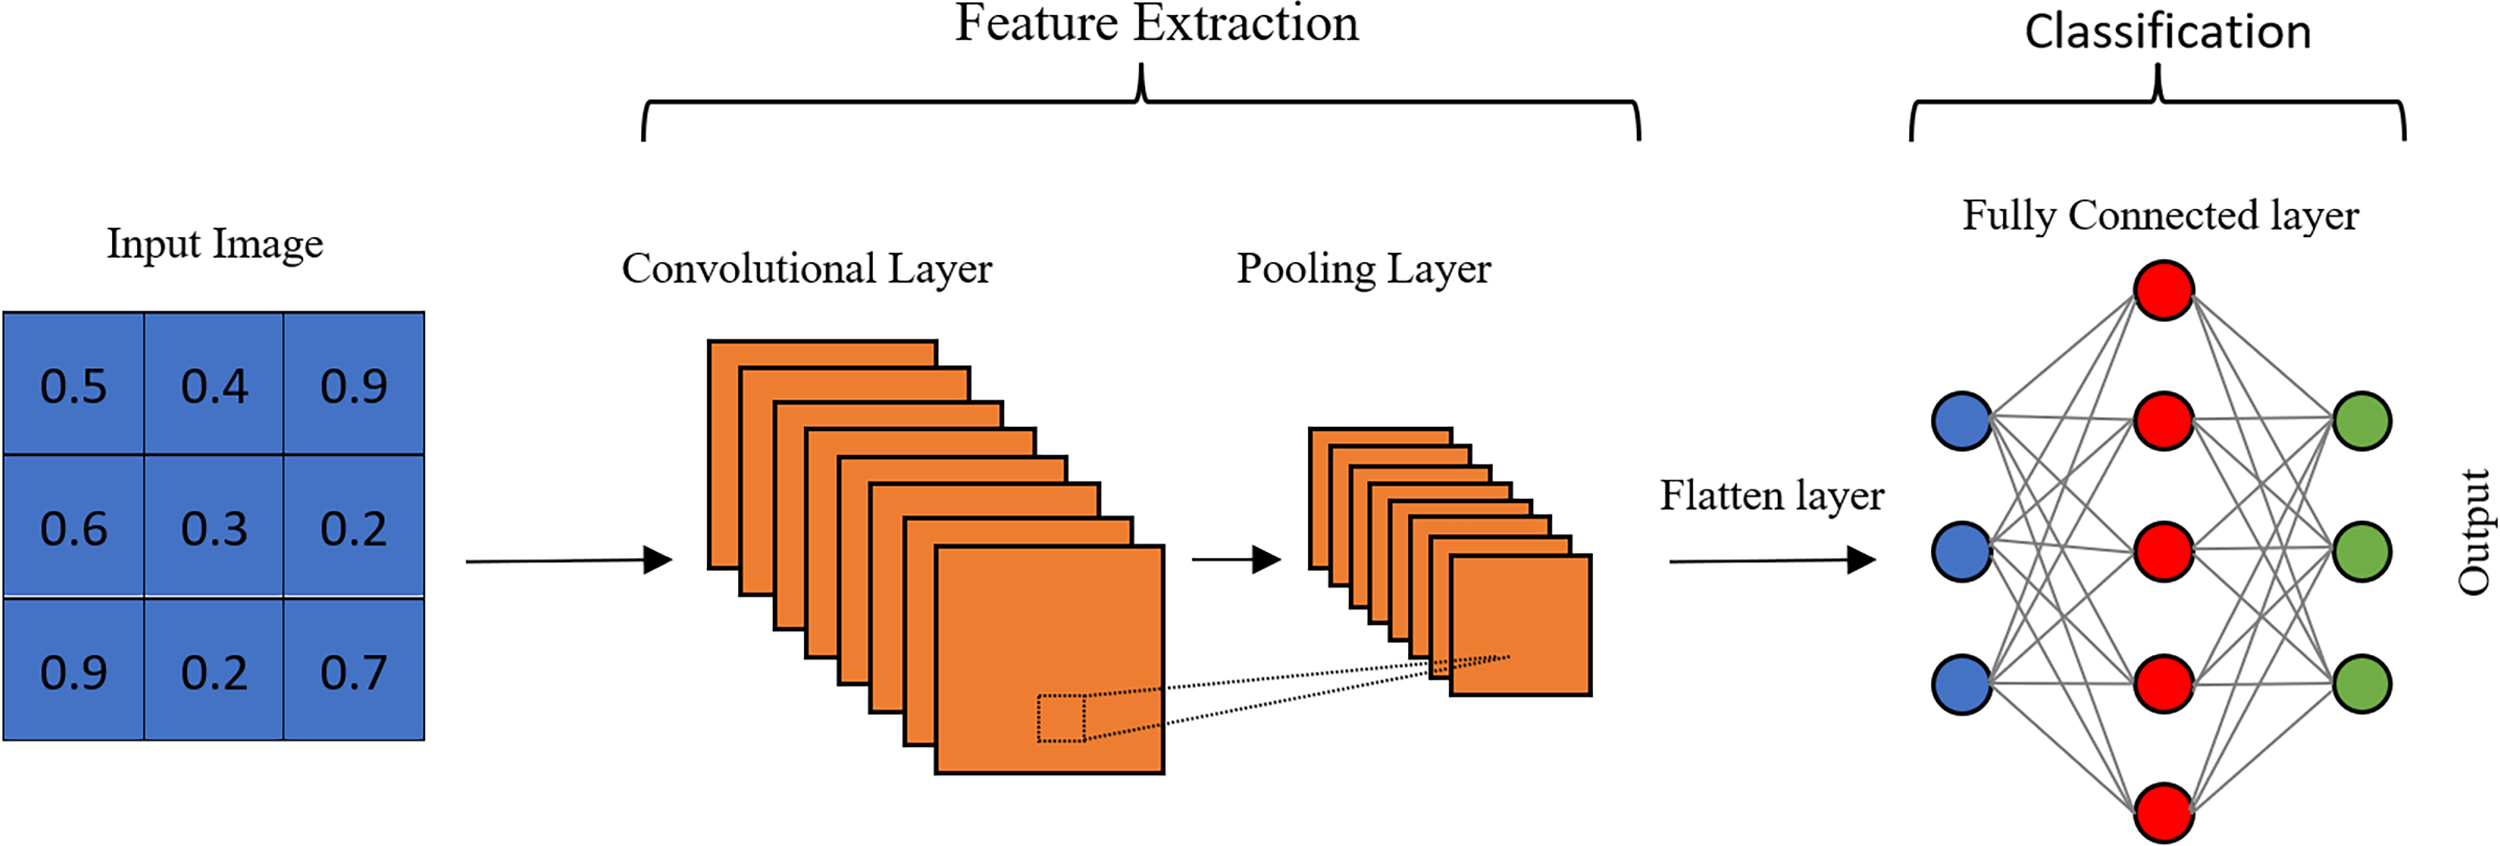
\includegraphics[width=0.95\textwidth]{images/cnn_structure}
    \caption{ساختار کلی یک شبکه عصبی کانولوشنی (CNN): ابتدا تصویر ورودی یا ماتریس ویژگی وارد شبکه می‌شود. در مرحله استخراج ویژگی، لایه‌های کانولوشنی و تجمعی به ترتیب ویژگی‌های محلی را استخراج و ابعاد داده را کاهش می‌دهند. سپس داده‌ها به یک بردار یک‌بعدی تبدیل شده (Flattening) و وارد لایه‌های کاملاً متصل می‌شوند تا فرایند طبقه‌بندی نهایی انجام گیرد. این ساختار باعث می‌شود شبکه بتواند به صورت خودکار و بدون نیاز به مهندسی ویژگی دستی، الگوهای پیچیده را شناسایی کند. برگرفته از \cite{Alsaleh2023}.}
    \label{fig:cnn_structure}
\end{figure}

\subsubsection{شبکه‌های عصبی بازگشتی و واحدهای حافظه بلند-کوتاه \lr{(RNN و LSTM)}}
شبکه‌های عصبی بازگشتی (\lr{Recurrent Neural Networks, RNNs}) نوعی از شبکه‌های عصبی هستند که به طور ویژه برای پردازش داده‌های ترتیبی و زمانی طراحی شده‌اند. برخلاف شبکه‌های پیش‌خور (\lr{Feedforward})، \lr{RNN}ها دارای حلقه‌های بازگشتی در اتصالات خود هستند که به آن‌ها اجازه می‌دهد اطلاعات مربوط به مراحل قبلی توالی را در یک حالت پنهان (\lr{Hidden State}) حفظ کرده و از آن برای پردازش مراحل بعدی استفاده کنند. این "حافظه" داخلی، \lr{RNN}ها را برای کاربردهایی مانند تحلیل توالی فراخوانی‌های \lr{API}، پردازش زبان طبیعی (مانند تحلیل کدهای اسمبلی یا توضیحات برنامه)، و تشخیص رفتارهای پویای اپلیکیشن‌ها که در طول زمان آشکار می‌شوند، مناسب می‌سازد.

یکی از چالش‌های اصلی \lr{RNN}های ساده، مشکل محو یا انفجار گرادیان (\lr{Vanishing/Exploding Gradient}) در هنگام یادگیری وابستگی‌های بلندمدت در توالی‌های طولانی است. برای رفع این مشکل، ساختارهای پیشرفته‌تری مانند واحد حافظه بلند-کوتاه (\lr{Long Short-Term Memory, LSTM}) \cite{Hochreiter1997} و واحد بازگشتی دروازه‌ای (\lr{Gated Recurrent Unit, GRU}) \cite{Cho2014} معرفی شده‌اند. \lr{LSTM} با بهره‌گیری از یک سلول حافظه (\lr{Memory Cell}) و سه نوع گیت (گیت فراموشی، گیت ورودی و گیت خروجی)، امکان کنترل دقیق جریان اطلاعات را فراهم می‌کند. این گیت‌ها به شبکه اجازه می‌دهند تا تصمیم بگیرد کدام اطلاعات را در سلول حافظه نگه دارد، کدام را فراموش کند و کدام را به عنوان خروجی مرحله فعلی استفاده کند. این مکانیزم به \lr{LSTM}ها کمک می‌کند تا اطلاعات مهم را در طول توالی‌های بسیار طولانی حفظ کرده و وابستگی‌های بلندمدت را به طور مؤثرتری مدل‌سازی کنند. \lr{GRU} ساختار ساده‌تری نسبت به \lr{LSTM} دارد (با دو گیت) اما عملکرد مشابهی در بسیاری از وظایف ارائه می‌دهد.

در این پژوهش، از \lr{LSTM} (یا می‌توانست از \lr{GRU} استفاده شود) برای تحلیل داده‌های ترتیبی، مانند توالی فراخوانی‌های \lr{API}، به منظور شناسایی الگوهای رفتاری پویا در اپلیکیشن‌های اندرویدی استفاده شده است. این قابلیت، \lr{LSTM} را به ابزاری قدرتمند برای تشخیص رفتارهای مخربی که در طول زمان و از طریق دنباله‌ای از اقدامات رخ می‌دهند، تبدیل می‌کند.

\subsubsection{شبکه‌های عصبی گرافی (GNN)}
شبکه‌های عصبی گرافی (\lr{Graph Neural Networks, GNNs}) دسته‌ای از مدل‌های یادگیری عمیق هستند که برای پردازش داده‌هایی با ساختار گرافی (مانند شبکه‌های اجتماعی، مولکول‌های شیمیایی، یا گراف‌های فراخوانی توابع در نرم‌افزار) طراحی شده‌اند \cite{sanchez-lengeling2021a}. داده‌های گرافی شامل مجموعه‌ای از گره‌ها (\lr{Nodes}) و لبه‌ها (\lr{Edges}) هستند که به ترتیب موجودیت‌ها و روابط بین آن‌ها را نشان می‌دهند. \lr{GNN}ها قادرند هم ساختار (توپولوژی) گراف و هم ویژگی‌های گره‌ها و لبه‌ها را برای یادگیری بازنمایی‌های مفید به کار گیرند.

ایده اصلی در \lr{GNN}ها، به‌روزرسانی بازنمایی (بردار ویژگی) هر گره بر اساس اطلاعات گره‌های همسایه آن است. این فرآیند معمولاً شامل دو مرحله اصلی است که در هر لایه \lr{GNN} تکرار می‌شود:
\begin{enumerate}
    \item \textbf{تجمیع \lr{(Aggregation)}:} جمع‌آوری اطلاعات (بازنمایی‌ها) از گره‌های همسایه. روش‌های مختلفی برای تجمیع وجود دارد، مانند میانگین‌گیری، جمع یا حداکثرگیری.
    \item \textbf{به‌روزرسانی \lr{(Update)}:} ترکیب اطلاعات تجمیع‌شده از همسایگان با اطلاعات خود گره (بازنمایی فعلی آن) برای تولید بازنمایی جدید گره. این کار معمولاً با استفاده از یک شبکه عصبی کوچک (مانند یک لایه خطی و یک تابع فعال‌سازی) انجام می‌شود.
\end{enumerate}
با پشته کردن چندین لایه \lr{GNN}، هر گره می‌تواند اطلاعات را از همسایگان دورتر نیز دریافت کند و بازنمایی‌های پیچیده‌تری که الگوهای ساختاری سطح بالاتر را در بر می‌گیرند، یاد گرفته شود.

در این پژوهش، از \lr{GNN} (به‌طور خاص، احتمالاً مدل‌هایی مانند \lr{Graph Convolutional Network (GCN)} \cite{Kipf2017} یا \lr{Graph Attention Network (GAT)} \cite{Velickovic2018}) برای تحلیل داده‌های گرافی استخراج‌شده از اپلیکیشن‌ها (مانند گراف فراخوانی \lr{API}) استفاده شده است. این داده‌ها با استفاده از کتابخانه \lr{torch\_geometric} به صورت اشیای \lr{Data} بارگذاری و پردازش می‌شوند. \lr{GNN}ها به مدل کمک می‌کنند تا ویژگی‌های ساختاری مهمی را که ممکن است نشان‌دهنده رفتار مخرب باشند (مانند الگوهای خاصی از تعامل بین توابع یا اجزا) استخراج کنند.

\begin{figure}[!t]
    \centering
    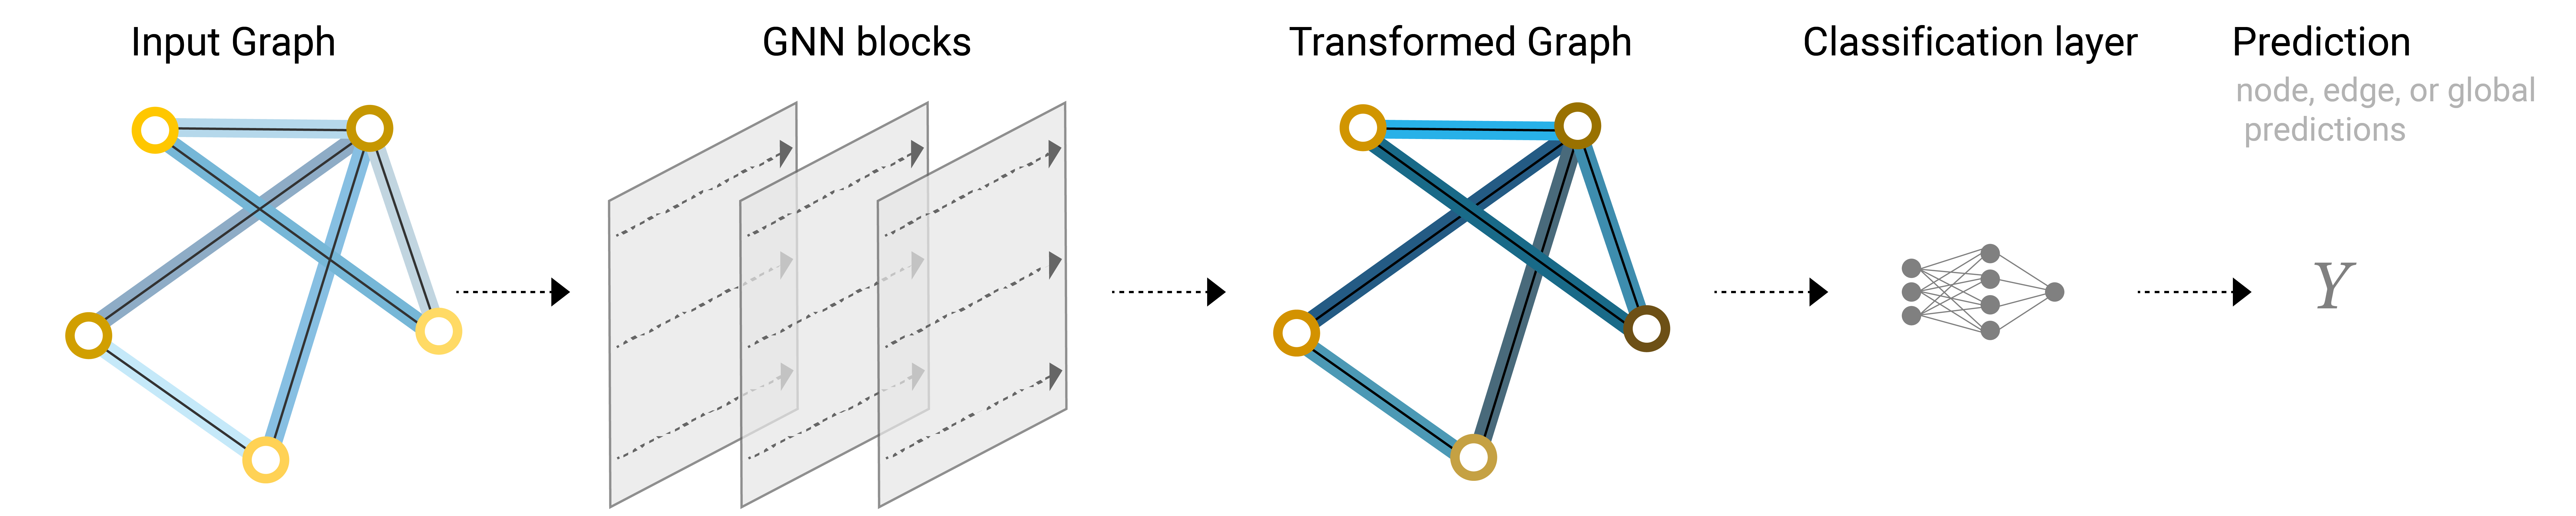
\includegraphics[width=0.95\textwidth]{images/gnn_structure}
    \caption{نمایی از یک مدل شبکه عصبی گرافی (GNN): ابتدا گراف ورودی (با ویژگی‌های اولیه گره‌ها و ساختار اتصالات) به مدل داده می‌شود. سپس در چندین بلوک GNN (لایه)، اطلاعات گره‌ها با تجمیع اطلاعات از همسایگان و به‌روزرسانی با استفاده از شبکه‌های عصبی کوچک، به‌طور مکرر پالایش می‌شود تا بازنمایی‌های غنی‌تری (گراف تبدیل‌شده) حاصل شود. در نهایت، این بازنمایی‌ها می‌توانند برای وظایف مختلف مانند طبقه‌بندی کل گراف (مثلاً بدافزار/سالم)، طبقه‌بندی گره‌ها (مثلاً شناسایی توابع مخرب) یا پیش‌بینی لبه‌ها استفاده شوند. برگرفته و بازطراحی‌شده بر اساس \cite{sanchez-lengeling2021a}.}
    \label{fig:gnn_structure}
\end{figure}

\subsection{ترنسفورمرها}

\paragraph{معرفی ترنسفورمر و تحول در مدل‌های یادگیری عمیق}
نقطه عطف برجسته‌ای در تکامل معماری‌های یادگیری عمیق، معرفی مدل ترنسفورمر در مقاله "\lr{Attention Is All You Need}" توسط \textcite{attention} بود که انقلابی در پردازش داده‌های ترتیبی، و بعدها انواع دیگر داده‌ها، به ارمغان آورد. این معماری، برخلاف مدل‌های بازگشتی (\lr{RNN/LSTM}) که توالی‌ها را به صورت مرحله به مرحله پردازش می‌کردند و با مشکلاتی مانند وابستگی‌های بلندمدت و عدم امکان پردازش موازی مواجه بودند، صرفاً بر مکانیزم توجه (\lr{Attention Mechanism})، به‌ویژه توجه خودی (\lr{Self-Attention}) و توجه چندسر (\lr{Multi-Head Attention})، تکیه می‌کند.

مکانیزم توجه به مدل اجازه می‌دهد تا هنگام پردازش یک عنصر در توالی (مثلاً یک کلمه در جمله یا یک فراخوانی \lr{API} در یک دنباله)، به طور مستقیم به تمام عناصر دیگر توالی نگاه کرده و وزن اهمیتی متفاوتی به هر یک اختصاص دهد. این قابلیت، مدل‌سازی وابستگی‌های بلندمدت بین عناصر را بسیار کارآمدتر می‌کند. همچنین، از آنجایی که محاسبات توجه برای هر عنصر می‌تواند به صورت موازی انجام شود، ترنسفورمرها سرعت آموزش و استنتاج را به‌طور چشمگیری بهبود بخشیدند و امکان آموزش مدل‌های بسیار بزرگتر را فراهم کردند. معماری استاندارد ترنسفورمر شامل دو بخش اصلی است: کدگذار (\lr{Encoder}) که ورودی را به یک دنباله از بازنمایی‌های پیوسته تبدیل می‌کند و گشاینده (\lr{Decoder}) که این بازنمایی‌ها را برای تولید خروجی (مثلاً در ترجمه ماشینی یا تولید متن) به کار می‌برد. هر دوی این بخش‌ها از پشته‌هایی از لایه‌های توجه چندسر و شبکه‌های عصبی پیش‌خور (\lr{Feed-Forward Networks}) تشکیل شده‌اند که با اتصالات باقیمانده (\lr{Residual Connections}) و نرمال‌سازی لایه‌ای (\lr{Layer Normalization}) ترکیب شده‌اند.

با ظهور ترنسفورمر، مدل‌های زبانی بزرگ (\lr{Large Language Models, LLMs}) پیشرفته‌ای مانند \lr{BERT} \cite{Devlin2019} (که از پشته کدگذار ترنسفورمر استفاده می‌کند و برای درک زبان آموزش دیده) و \lr{GPT} \cite{Radford2018, Radford2019, Brown2020} (که از پشته گشاینده ترنسفورمر بهره می‌برد و برای تولید زبان آموزش دیده) توسعه یافتند. این مدل‌ها با پیش‌آموزش روی حجم عظیمی از داده‌های متنی و سپس تنظیم دقیق (\lr{Fine-tuning}) برای وظایف خاص، عملکردی استثنایی در طیف وسیعی از کاربردهای پردازش زبان طبیعی نشان دادند.

این پیشرفت‌ها، الهام‌بخش کاربرد ترنسفورمرها در حوزه‌های فراتر از زبان، از جمله بینایی کامپیوتر (\lr{Vision Transformer}) \cite{Dosovitskiy2021}، تحلیل داده‌های گرافی \cite{Yun2019} و همچنین امنیت سایبری و تشخیص بدافزار \cite{TransformerMalware} شد. توانایی ترنسفورمر در مدل‌سازی روابط پیچیده و بلندمدت و پردازش موازی، آن را به گزینه‌ای جذاب برای تحلیل داده‌های چندوجهی و پیچیده مرتبط با بدافزارها تبدیل کرد.

\subsection{ترنسفورمرها در مدل MAGNET}
در این پژوهش، معماری ترنسفورمر به‌عنوان هسته اصلی مدل \lr{MAGNET} (\lr{Multi-Modal Analysis for Graph and Network Threat Detection}) به کار گرفته شده است تا داده‌های چندوجهی شامل داده‌های جدولی (ویژگی‌های ایستا)، گرافی (روابط ساختاری) و ترتیبی (رفتار پویا) را به‌صورت یکپارچه تحلیل کند. ترنسفورمر در این مدل از مکانیزم توجه پویا برای یادگیری بازنمایی‌های غنی (\lr{Embeddings}) از هر وجه داده و سپس تلفیق (\lr{Fusion}) هوشمندانه این بازنمایی‌ها استفاده می‌کند.

به‌طور خاص، لایه‌های کدگذار ترنسفورمر می‌توانند برای پردازش ویژگی‌های استخراج‌شده از داده‌های جدولی (پس از تبدیل به دنباله‌ای از ویژگی‌ها یا استفاده از توکن‌های خاص) و داده‌های گرافی (با استفاده از تکنیک‌هایی مانند تبدیل گره‌ها به دنباله یا به‌کارگیری \lr{Graph Transformers}) به کار روند. مکانیزم توجه چندسر به مدل اجازه می‌دهد تا روابط متقابل بین ویژگی‌های مختلف ایستا و ساختاری را کشف کند. همزمان، لایه‌های گشاینده ترنسفورمر (یا یک پشته کدگذار دیگر) می‌توانند برای مدل‌سازی توالی‌های ترتیبی (مانند فراخوانی‌های \lr{API}) به کار گرفته شوند تا الگوهای زمانی مخرب شناسایی شوند.

ساختار ترنسفورمر در \lr{MAGNET} احتمالاً شامل چندین بلوک کدگذار/گشاینده است که هر بلوک دارای یک لایه توجه چندسر و یک لایه تغذیه روبه‌جلو است. داده‌های ورودی از هر وجه ابتدا با استفاده از لایه‌های جاسازی (\lr{Embedding layers}، مانند \lr{nn.Embedding} در \lr{PyTorch} یا پروجکشن‌های خطی) به بردارهایی با ابعاد ثابت تبدیل می‌شوند. سپس، مکانیزم توجه خودی و احتمالاً توجه متقابل (\lr{Cross-Attention}) بین وجه‌های مختلف، وزن‌های متفاوتی به هر عنصر داده تخصیص می‌دهد تا اهمیت نسبی آن را در پیش‌بینی نهایی برچسب (سالم یا مخرب) تعیین کند. این فرآیند با استفاده از نرمال‌سازی لایه‌ای و اتصالات باقیمانده برای پایداری و بهبود آموزش، بهینه می‌شود.

مزیت اصلی استفاده از ترنسفورمر در مدل \lr{MAGNET}، توانایی آن در پردازش موازی داده‌های چندوجهی و درک روابط پیچیده و بلندمدت *درون* هر وجه و *بین* وجه‌های مختلف داده است. این ویژگی، به‌ویژه در شناسایی بدافزارهای پیچیده و ناشناخته که ممکن است از تکنیک‌های پنهان‌سازی پیشرفته استفاده کنند و نیازمند تحلیل جامع رفتار و ساختار اپلیکیشن‌ها هستند، بسیار مؤثر است. نتایج ادعا شده در متن (دقت \lr{۹۷.۲۴} درصد و \lr{F1 Score} \lr{۰.۹۸۲۳}) نشان می‌دهد که این رویکرد مبتنی بر ترنسفورمر و داده‌های چندوجهی، پتانسیل ارائه عملکردی برتر نسبت به مدل‌های سنتی یا تک‌وجهی را دارد.

\begin{figure}[!t]
    \centering
    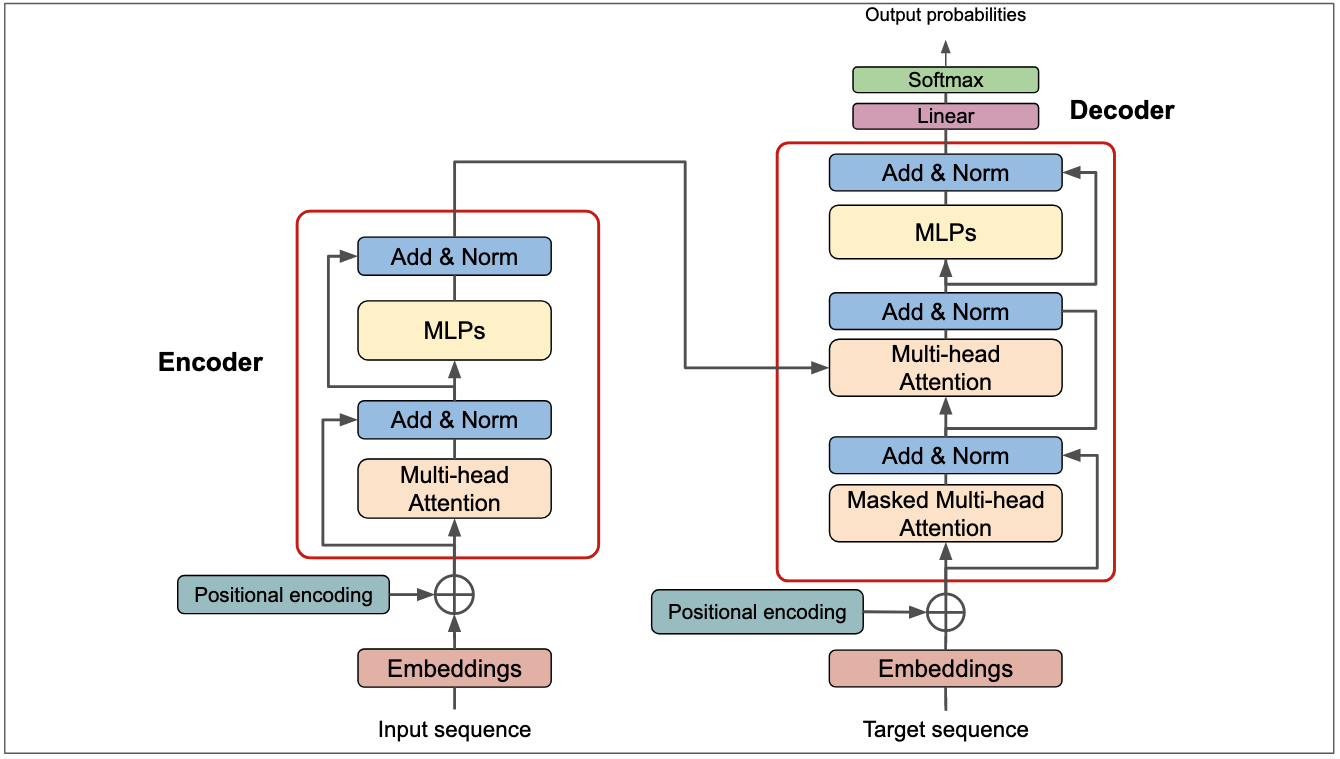
\includegraphics[width=0.95\textwidth]{images/transformer_structure}
    \caption{ساختار کلی معماری ترنسفورمر شامل بخش کدگذار (Encoder) در سمت چپ و گشاینده (Decoder) در سمت راست. هر دو بخش از پشته‌ای از لایه‌های یکسان تشکیل شده‌اند که عمدتاً شامل مکانیزم توجه چندسر (Multi-Head Attention) و شبکه‌های عصبی پیش‌خور (Feed Forward) هستند. اتصالات باقیمانده (Add) و نرمال‌سازی لایه‌ای (Norm) نیز برای پایداری آموزش استفاده می‌شوند. گشاینده علاوه بر توجه خودی، از توجه متقابل (Cross-Attention) برای در نظر گرفتن خروجی کدگذار نیز بهره می‌برد. این معماری امکان پردازش موازی و مدل‌سازی وابستگی‌های بلندمدت را فراهم می‌کند. برگرفته و بازطراحی‌شده بر اساس \cite{attention}.}
    \label{fig:transformer_structure}
\end{figure}

\subsection{ماشین بردار پشتیبان (SVM)}
ماشین بردار پشتیبان (\lr{Support Vector Machine, SVM}) یکی از الگوریتم‌های یادگیری نظارت‌شده قدرتمند و پرکاربرد است که عمدتاً برای مسائل طبقه‌بندی (\lr{Classification}) و همچنین رگرسیون (\lr{Regression}) استفاده می‌شود. ایده اصلی \lr{SVM} در مسائل طبقه‌بندی دودویی، یافتن یک ابرصفحه (\lr{Hyperplane}) بهینه در فضای ویژگی‌هاست که بتواند داده‌های مربوط به دو کلاس مختلف را به بهترین شکل ممکن از یکدیگر جدا کند.

"بهترین شکل ممکن" در \lr{SVM} به معنای یافتن ابرصفحه‌ای است که بیشترین حاشیه (\lr{Margin}) را با نزدیک‌ترین نقاط داده از هر دو کلاس داشته باشد. این نزدیک‌ترین نقاط، که روی مرز حاشیه قرار می‌گیرند، بردارهای پشتیبان (\lr{Support Vectors}) نامیده می‌شوند، زیرا موقعیت ابرصفحه جداکننده تنها به این نقاط بستگی دارد. هدف، حداکثر کردن این حاشیه است، زیرا تئوری یادگیری آماری نشان می‌دهد که جداکننده‌ای با حاشیه بزرگتر، معمولاً خطای تعمیم کمتری دارد و عملکرد بهتری روی داده‌های دیده‌نشده خواهد داشت.

\paragraph{انواع SVM}
\begin{itemize}
    \item \textbf{SVM خطی \lr{(Linear SVM)}:} زمانی که داده‌ها به صورت خطی قابل تفکیک باشند (یعنی بتوان با یک خط مستقیم یا یک صفحه صاف آن‌ها را جدا کرد)، از \lr{SVM} خطی استفاده می‌شود.
    \item \textbf{SVM غیرخطی \lr{(Non-linear SVM)}:} در بسیاری از مسائل دنیای واقعی، داده‌ها به صورت خطی قابل تفکیک نیستند. در این موارد، \lr{SVM} از ترفند کرنل (\lr{Kernel Trick}) استفاده می‌کند. ترفند کرنل به \lr{SVM} اجازه می‌دهد تا داده‌ها را به یک فضای ویژگی با ابعاد بالاتر نگاشت کند که در آن، داده‌ها ممکن است به صورت خطی قابل تفکیک شوند. سپس \lr{SVM} خطی در آن فضای جدید اعمال می‌شود. توابع کرنل رایج شامل کرنل چندجمله‌ای (\lr{Polynomial})، کرنل تابع پایه شعاعی (\lr{Radial Basis Function, RBF}) یا گاوسی، و کرنل سیگموئید (\lr{Sigmoid}) هستند.
\end{itemize}

\paragraph{کاربرد در تشخیص بدافزار}
\lr{SVM} به دلیل عملکرد خوب در فضاهای با ابعاد بالا و مقاومت نسبی در برابر بیش‌برازش (\lr{Overfitting})، به‌طور گسترده‌ای در تشخیص بدافزار اندروید، به‌ویژه با استفاده از ویژگی‌های استاتیک (مانند مجوزها، فراخوانی‌های \lr{API}) یا ویژگی‌های پویا (مانند توالی‌های رفتاری) استفاده شده است \cite{AndroidMalwareSurvey, Demontis2017}. اغلب، ویژگی‌های استخراج‌شده از اپلیکیشن‌ها به عنوان ورودی به \lr{SVM} داده می‌شوند تا مدل آموزش ببیند که آیا یک اپلیکیشن بدافزار است یا خیر.

\paragraph{مزایا و معایب}
\begin{itemize}
    \item \textbf{مزایا:} کارایی بالا در فضاهای با ابعاد زیاد، مؤثر بودن در مواردی که تعداد ابعاد بیشتر از تعداد نمونه‌هاست، حافظه کارآمد (چون فقط از بردارهای پشتیبان استفاده می‌کند)، تطبیق‌پذیری با استفاده از کرنل‌های مختلف.
    \item \textbf{معایب:} عملکرد ضعیف در مجموعه داده‌های بسیار بزرگ (به دلیل پیچیدگی محاسباتی آموزش که می‌تواند بین \(O(n^2)\) تا \(O(n^3)\) باشد)، حساسیت به انتخاب تابع کرنل و پارامترهای آن (مانند پارامتر C یا هزینه خطا و پارامتر گاما در کرنل RBF)، عدم ارائه مستقیم احتمالات تعلق به کلاس (اگرچه روش‌هایی برای تخمین آن وجود دارد).
\end{itemize}
اگرچه مدل‌های یادگیری عمیق مانند \lr{CNN} و ترنسفورمرها در سال‌های اخیر توجه بیشتری را به خود جلب کرده‌اند، \lr{SVM} همچنان یک ابزار قدرتمند و یک معیار (\lr{Baseline}) مهم در حوزه تشخیص بدافزار محسوب می‌شود.

\section{تکنیک‌های آموزشی و ارزیابی}
در این بخش، تکنیک‌های کلیدی مورد استفاده برای آموزش مدل \lr{MAGNET} و ارزیابی عملکرد آن تشریح می‌شود. این تکنیک‌ها برای اطمینان از قابلیت اطمینان، کارایی و تعمیم‌پذیری مدل ضروری هستند.

\subsection{اعتبارسنجی متقاطع (Cross-Validation)}
اعتبارسنجی متقاطع (\lr{Cross-Validation}) یک تکنیک آماری برای ارزیابی عملکرد مدل‌های یادگیری ماشین و تخمین میزان تعمیم‌پذیری آن‌ها به داده‌های جدید و مستقل است. این روش به کاهش واریانس تخمین عملکرد کمک کرده و از بیش‌برازش (\lr{Overfitting}) بر روی یک تقسیم خاص از داده‌ها به مجموعه‌های آموزشی و آزمایشی جلوگیری می‌کند.

رایج‌ترین نوع اعتبارسنجی متقاطع، \textbf{اعتبارسنجی {k-تایی} \lr{(k-fold Cross-Validation)}} است. در این روش:
\begin{enumerate}
    \item مجموعه داده اصلی به صورت تصادفی به \lr{k} زیرمجموعه (یا "تا") با اندازه تقریباً مساوی تقسیم می‌شود.
    \item فرآیند آموزش و ارزیابی \lr{k} بار تکرار می‌شود.
    \item در هر تکرار (\lr{i} از ۱ تا \lr{k})، از \lr{k-1} زیرمجموعه برای آموزش مدل استفاده می‌شود و از زیرمجموعه باقی‌مانده (تا \lr{i}-ام) به عنوان مجموعه اعتبارسنجی (\lr{Validation Set}) برای ارزیابی مدل استفاده می‌شود.
    \item نتایج ارزیابی (مانند دقت، \lr{F1 Score}) از هر \lr{k} تکرار جمع‌آوری می‌شود.
    \item میانگین (و گاهی انحراف معیار) این نتایج به عنوان تخمین نهایی عملکرد مدل گزارش می‌شود.
\end{enumerate}
در این پژوهش، از \textbf{اعتبارسنجی ۵-تایی \lr{(5-fold Cross-Validation)}} استفاده شده است (\(k=5\)). این بدان معناست که داده‌ها به پنج بخش تقسیم شده و مدل پنج بار آموزش و ارزیابی می‌شود، هر بار با یک بخش متفاوت به عنوان داده اعتبارسنجی. این رویکرد نسبت به تقسیم ساده آموزشی/آزمایشی، تخمین پایدارتر و قابل اعتمادتری از عملکرد مدل ارائه می‌دهد، زیرا از تمام داده‌ها هم برای آموزش و هم برای ارزیابی استفاده می‌شود. در پیاده‌سازی کد، این فرآیند می‌تواند با استفاده از توابعی مانند \lr{KFold} یا \lr{StratifiedKFold} از کتابخانه \lr{scikit-learn} و اجرای حلقه آموزش و ارزیابی (مانند تابع فرضی \lr{train\_and\_evaluate\_magnet}) در هر تقسیم انجام شود.

\subsection{مدیریت اورفیتینگ و آندرفیتینگ}
دو چالش اساسی در آموزش مدل‌های یادگیری ماشین، به‌ویژه مدل‌های یادگیری عمیق با ظرفیت بالا، بیش‌برازش (\lr{Overfitting}) و کم‌برازش (\lr{Underfitting}) هستند.

\begin{itemize}
    \item \textbf{کم‌برازش \lr{(Underfitting)}:} زمانی رخ می‌دهد که مدل به اندازه کافی پیچیده نیست یا به اندازه کافی آموزش ندیده است تا الگوهای اساسی موجود در داده‌های آموزشی را یاد بگیرد. در نتیجه، مدل هم بر روی داده‌های آموزشی و هم بر روی داده‌های جدید عملکرد ضعیفی دارد. برای مقابله با کم‌برازش، می‌توان پیچیدگی مدل را افزایش داد (مثلاً با افزودن لایه‌ها یا نورون‌ها)، ویژگی‌های بهتری مهندسی کرد، یا زمان آموزش را افزایش داد. در مدل \lr{MAGNET}، تنظیم مناسب تعداد لایه‌ها (\lr{num\_layers}) و ابعاد نهان (\lr{embedding\_dim}) می‌تواند به جلوگیری از کم‌برازش کمک کند.
    \item \textbf{بیش‌برازش \lr{(Overfitting)}:} زمانی رخ می‌دهد که مدل بیش از حد به داده‌های آموزشی خاص، از جمله نویز و جزئیات تصادفی آن، وابسته می‌شود. در نتیجه، مدل بر روی داده‌های آموزشی عملکرد بسیار خوبی دارد، اما توانایی تعمیم به داده‌های جدید و دیده‌نشده را از دست می‌دهد و بر روی آن‌ها عملکرد ضعیفی نشان می‌دهد. برای مقابله با بیش‌برازش، از تکنیک‌های تنظیم‌گری (\lr{Regularization}) استفاده می‌شود. در این پژوهش، از تکنیک‌های زیر استفاده شده است:
    \begin{itemize}
        \item \textbf{\lr{Dropout}:} در هر مرحله آموزش، به طور تصادفی برخی از نورون‌ها (و اتصالات آن‌ها) را با احتمال مشخصی (در اینجا با نرخ ۰.۲) غیرفعال می‌کند. این کار باعث می‌شود شبکه به یک مسیر یا ویژگی خاص بیش از حد وابسته نشود و مدل مقاوم‌تری یاد بگیرد.
        \item \textbf{توقف زودهنگام \lr{(Early Stopping)}:} عملکرد مدل بر روی یک مجموعه اعتبارسنجی جداگانه در طول آموزش نظارت می‌شود. اگر عملکرد مدل روی مجموعه اعتبارسنجی برای تعداد مشخصی از دوره‌ها (Epochs) بهبود نیابد (در اینجا با صبر ۳ دوره)، آموزش متوقف می‌شود، حتی اگر عملکرد روی مجموعه آموزشی همچنان در حال بهبود باشد. این کار از ادامه آموزش و ورود مدل به فاز بیش‌برازش جلوگیری می‌کند.
        \item \textbf{تنظیم‌گری L2 \lr{(Weight Decay)}:} (هرچند به صراحت در بخش بیش‌برازش ذکر نشده، اما در بخش بهینه‌سازی Adam با \lr{{weight\_decay}=۰.۰۱} اشاره شده است). این روش با افزودن یک جمله جریمه به تابع هزینه که متناسب با مجذور اندازه وزن‌های مدل است، از بزرگ شدن بیش از حد وزن‌ها جلوگیری می‌کند و به مدل ساده‌تر و با تعمیم‌پذیری بهتر منجر می‌شود.
    \end{itemize}
\end{itemize}
تحلیل نمودارهای تابع هزینه و معیارهای ارزیابی بر روی داده‌های آموزشی و اعتبارسنجی در طول زمان آموزش، ابزار مهمی برای تشخیص و مدیریت این دو پدیده است.

\subsection{روش‌های بهینه‌سازی}
بهینه‌سازی فرآیند تنظیم پارامترهای مدل (مانند وزن‌ها و بایاس‌ها در شبکه‌های عصبی) به منظور کمینه کردن تابع هزینه (\lr{Loss Function}) است. انتخاب الگوریتم بهینه‌سازی مناسب و تنظیم ابرپارامترهای (\lr{Hyperparameters}) آن نقش کلیدی در سرعت همگرایی و کیفیت نهایی مدل دارد.

\subsubsection{الگوریتم Adam}
الگوریتم \lr{Adam} (\lr{Adaptive Moment Estimation}) \cite{Kingma2015} یکی از محبوب‌ترین و کارآمدترین الگوریتم‌های بهینه‌سازی مبتنی بر گرادیان نزولی تصادفی (\lr{Stochastic Gradient Descent, SGD}) است که برای آموزش شبکه‌های عصبی عمیق استفاده می‌شود. \lr{Adam} نرخ یادگیری (\lr{Learning Rate}) را برای هر پارامتر به صورت تطبیقی تنظیم می‌کند. این کار را با استفاده از تخمین‌های مرتبه اول (میانگین یا مومنتوم) و مرتبه دوم (واریانس غیرمرکزی) گرادیان‌ها انجام می‌دهد. به عبارت دیگر، \lr{Adam} مزایای دو الگوریتم دیگر، یعنی \lr{AdaGrad} (که نرخ یادگیری را بر اساس فراوانی به‌روزرسانی پارامتر تنظیم می‌کند) و \lr{RMSProp} (که از میانگین متحرک نمایی مجذور گرادیان‌ها استفاده می‌کند) را با هم ترکیب می‌کند و همچنین از مومنتوم برای هموارسازی مسیر گرادیان و تسریع همگرایی بهره می‌برد.
در این پژوهش، \lr{Adam} با نرخ یادگیری پیش‌فرض (معمولاً \lr{۰.۰۰۱}) و ضریب تنظیم‌گری \lr{L2} (\lr{weight\_decay}) برابر با \lr{۰.۰۱} در تابع \lr{train\_and\_evaluate\_magnet} برای به‌روزرسانی وزن‌های مدل \lr{MAGNET} به کار رفته است. \lr{Adam} به دلیل سرعت همگرایی بالا، نیاز کمتر به تنظیم دقیق نرخ یادگیری اولیه، و عملکرد خوب در مسائل با گرادیان‌های پراکنده یا نویزی، انتخاب مناسبی برای آموزش مدل‌های پیچیده مانند ترنسفورمر و \lr{GNN} بر روی داده‌های چندوجهی بوده است.

\subsubsection{الگوریتم PIRATES}
الگوریتم \lr{PIRATES}\LTRfootnote{Pirate-Inspired Robust Adaptive Trajectory Exploration Strategy} یکی از روش‌های نوین بهینه‌سازی الهام‌گرفته از طبیعت است که با الهام از رفتار جمعی دزدان دریایی در جستجوی گنج طراحی شده است. در این الگوریتم، هر راه‌حل بالقوه به عنوان یک «کشتی» در فضای جستجو مدل می‌شود و مجموعه‌ای از کشتی‌ها (جمعیت) به طور موازی و با استفاده از اطلاعات فردی (تجربیات گذشته)، جمعی (اطلاعات بهترین اعضا)، و تعاملات خاص (مانند نبرد و طوفان)، به سمت نقاط بهینه حرکت می‌کنند. این الگوریتم با ترکیب ایده‌هایی از الگوریتم‌های ازدحامی (مانند PSO) و تکاملی، سعی در افزایش پایداری، سرعت همگرایی و جلوگیری از گیر افتادن در بهینه‌های محلی دارد.

اجزای کلیدی این الگوریتم عبارت‌اند از:
\begin{itemize}
    \item \textbf{کشتی‌ها \lr{(Ships)}:} هر کشتی نمایانگر یک نقطه در فضای جستجو است و موقعیت و سرعت مخصوص به خود را دارد.
    \item \textbf{رهبر \lr{(Leader)}:} کشتی با بهترین عملکرد (کمترین مقدار تابع هدف) در هر تکرار به عنوان رهبر انتخاب می‌شود و سایر کشتی‌ها از آن پیروی می‌کنند.
    \item \textbf{نقشه جمعی و خصوصی:} هر کشتی علاوه بر بهترین موقعیت شخصی، از نقشه‌ای جمعی (شامل بهترین موقعیت‌های سایر کشتی‌ها) نیز بهره می‌برد.
    \item \textbf{کشتی‌های برتر \lr{(Top Ships)}:} تعدادی از بهترین کشتی‌ها به عنوان مرجع برای سایر اعضا عمل می‌کنند.
    \item \textbf{مکانیزم‌های تنوع‌بخش:} الگوریتم با استفاده از نبرد بین کشتی‌های برتر و وقوع طوفان‌های تصادفی، از همگرایی زودهنگام و گیر افتادن در بهینه‌های محلی جلوگیری می‌کند.
\end{itemize}

الگوریتم PIRATES با بهره‌گیری از چندین منبع اطلاعاتی و تنظیم پویا، قادر است به سرعت به نقاط بهینه همگرا شود و در عین حال تنوع جمعیت را حفظ کند. این ویژگی‌ها، PIRATES را به گزینه‌ای مناسب برای بهینه‌سازی مسائل پیچیده، از جمله تنظیم خودکار هایپرپارامترهای مدل‌های یادگیری عمیق و چندوجهی، تبدیل کرده است. در پژوهش حاضر، از این الگوریتم برای جستجوی بهینه پارامترهای مدل پیشنهادی (MAGNET) استفاده شده است تا عملکرد مدل در تشخیص بدافزارهای اندرویدی بهبود یابد.

استفاده از الگوریتم‌های بهینه‌سازی الهام‌گرفته از طبیعت، به ویژه \lr{PIRATES}، در سال‌های اخیر به عنوان رویکردی مؤثر برای حل مسائل بهینه‌سازی غیرخطی و پیچیده در حوزه‌های مختلف، از جمله امنیت سایبری و یادگیری ماشین، مطرح شده است. در این پژوهش، PIRATES به عنوان یکی از ابزارهای کلیدی برای تنظیم بهینه پارامترهای مدل چندوجهی مبتنی بر ترنسفورمر و شبکه‌های عصبی گرافی به کار رفته است.

\subsubsection{الگوریتم Optuna}
\lr{Optuna} \cite{Optuna2019} یک چارچوب (\lr{Framework}) نرم‌افزاری متن‌باز و قدرتمند برای بهینه‌سازی خودکار هایپرپارامترها است. \lr{Optuna} از الگوریتم‌های جستجوی متنوعی پشتیبانی می‌کند، از جمله جستجوی تصادفی (\lr{Random Search})، جستجوی شبکه‌ای (\lr{Grid Search})، و الگوریتم‌های پیشرفته‌تر مبتنی بر مدل مانند \lr{Tree-structured Parzen Estimator (TPE)} که نوعی بهینه‌سازی بیزی است. یکی از ویژگی‌های کلیدی \lr{Optuna}، قابلیت هرس (\lr{Pruning}) آزمایش‌های ناموفق است. با استفاده از الگوریتم‌های هرس (مانند \lr{Median Pruning} یا \lr{Successive Halving})، \lr{Optuna} می‌تواند آزمایش‌هایی را که در مراحل اولیه عملکرد ضعیفی دارند، متوقف کرده و منابع محاسباتی را بر روی آزمایش‌های امیدوارکننده‌تر متمرکز کند.

در این پژوهش، ادعا شده که از \lr{Optuna} برای تنظیم پارامترهایی مانند نرخ \lr{Dropout} (که مقدار بهینه ۰.۲ یافت شده) و ابعاد نهان (\lr{embedding\_dim}) استفاده شده است. این فرآیند معمولاً شامل تعریف یک تابع هدف (مانند تابع \lr{train\_and\_evaluate\_magnet} که یک معیار عملکرد مثل \lr{F1 Score} یا دقت را برمی‌گرداند) و مشخص کردن فضای جستجو برای هر هایپرپارامتر است. سپس \lr{Optuna} با اجرای مکرر تابع هدف با مقادیر مختلف هایپرپارامترها (که با استفاده از نمونه‌برداری تطبیقی انتخاب می‌شوند)، به تدریج به سمت یافتن ترکیب بهینه حرکت می‌کند. استفاده از \lr{Optuna} می‌تواند فرآیند زمان‌بر و خسته‌کننده تنظیم دستی هایپرپارامترها را خودکار کرده و به یافتن مدل‌هایی با عملکرد بهتر کمک کند.

\subsection{معیارهای ارزیابی عملکرد}
برای ارزیابی کمی و کیفی عملکرد مدل طبقه‌بندی \lr{MAGNET} در تشخیص بدافزارهای اندرویدی، از معیارهای استاندارد مختلفی استفاده شده است. انتخاب معیار مناسب به ماهیت مسئله و توزیع کلاس‌ها در مجموعه داده بستگی دارد.

\subsubsection{دقت (Accuracy)}
دقت (\lr{Accuracy}) ساده‌ترین و رایج‌ترین معیار ارزیابی است که نسبت کل نمونه‌هایی که به درستی توسط مدل طبقه‌بندی شده‌اند (چه مثبت و چه منفی) به تعداد کل نمونه‌ها را اندازه‌گیری می‌کند:
\[ \text{Accuracy} = \frac{\text{TP} + \text{TN}}{\text{TP} + \text{TN} + \text{FP} + \text{FN}} \]
که در آن:
\begin{itemize}
    \item \lr{TP (True Positive)}: تعداد نمونه‌های بدافزار که به درستی بدافزار تشخیص داده شده‌اند.
    \item \lr{TN (True Negative)}: تعداد نمونه‌های سالم که به درستی سالم تشخیص داده شده‌اند.
    \item \lr{FP (False Positive)}: تعداد نمونه‌های سالم که به اشتباه بدافزار تشخیص داده شده‌اند (خطای نوع اول).
    \item \lr{FN (False Negative)}: تعداد نمونه‌های بدافزار که به اشتباه سالم تشخیص داده شده‌اند (خطای نوع دوم).
\end{itemize}
در این پژوهش، دقت مدل \lr{MAGNET} در تست نهایی ۹۷.۲۴ درصد گزارش شده است. دقت معیار خوبی است زمانی که کلاس‌ها تقریباً متوازن باشند. با این حال، در مجموعه‌های داده نامتوازن (مثلاً اگر تعداد نمونه‌های سالم بسیار بیشتر از بدافزارها باشد)، دقت بالا ممکن است گمراه‌کننده باشد.

\subsubsection{F1 Score}
امتیاز \lr{F1} (\lr{F1 Score}) میانگین هارمونیک دو معیار دیگر، یعنی دقت (\lr{Precision}) و یادآوری (\lr{Recall}) است و به ویژه در مسائل با کلاس‌های نامتوازن مفید است.
\begin{itemize}
    \item \textbf{دقت \lr{(Precision)}:} نسبت نمونه‌هایی که به درستی مثبت پیش‌بینی شده‌اند به کل نمونه‌هایی که مثبت پیش‌بینی شده‌اند. این معیار نشان می‌دهد که چقدر می‌توان به پیش‌بینی‌های مثبت مدل اعتماد کرد.
    \[ \text{Precision} = \frac{\text{TP}}{\text{TP} + \text{FP}} \]
    \item \textbf{یادآوری (Recall) یا حساسیت (Sensitivity) یا نرخ مثبت واقعی \lr{(TPR)}:} نسبت نمونه‌هایی که به درستی مثبت پیش‌بینی شده‌اند به کل نمونه‌های واقعاً مثبت. این معیار نشان می‌دهد که مدل چه کسری از نمونه‌های مثبت واقعی را توانسته شناسایی کند.
    \[ \text{Recall} = \frac{\text{TP}}{\text{TP} + \text{FN}} \]
\end{itemize}
امتیاز \lr{F1} به صورت زیر محاسبه می‌شود:
\[ \text{F1 Score} = 2 \times \frac{\text{Precision} \times \text{Recall}}{\text{Precision} + \text{Recall}} = \frac{2 \times \text{TP}}{2 \times \text{TP} + \text{FP} + \text{FN}} \]
امتیاز \lr{F1} تعادلی بین دقت و یادآوری برقرار می‌کند و مقدار بالای آن نشان می‌دهد که مدل هم در کاهش هشدارهای کاذب (\lr{FP} بالا باعث کاهش \lr{Precision} می‌شود) و هم در شناسایی نمونه‌های مثبت واقعی (\lr{FN} بالا باعث کاهش \lr{Recall} می‌شود) موفق بوده است. در این پژوهش، مقدار \lr{F1 Score} \lr{۰.۹۸۲۳} در بهترین حالت به دست آمده که نشان‌دهنده عملکرد بسیار خوب مدل در هر دو جنبه است. این معیار معمولاً برای ارزیابی عملکرد در تشخیص بدافزار ارجحیت دارد، زیرا هزینه تشخیص نادرست (\lr{FN} یا \lr{FP}) می‌تواند بالا باشد.

\subsubsection{AUC \lr{(Area Under the ROC Curve)}}
منحنی مشخصه عملکرد گیرنده (\lr{Receiver Operating Characteristic, ROC}) نموداری است که نرخ مثبت واقعی (\lr{True Positive Rate, TPR} یا همان \lr{Recall}) را در مقابل نرخ مثبت کاذب (\lr{False Positive Rate, FPR}) در آستانه‌های طبقه‌بندی مختلف رسم می‌کند.
\[ \text{FPR} = \frac{\text{FP}}{\text{FP} + \text{TN}} \]
مساحت زیر این منحنی (\lr{Area Under the Curve, AUC}) یک معیار واحد است که توانایی کلی مدل در تمایز بین کلاس‌های مثبت و منفی را در تمام آستانه‌های ممکن اندازه‌گیری می‌کند. مقدار \lr{AUC} بین ۰ و ۱ متغیر است.
\begin{itemize}
    \item \lr{AUC = 1}: طبقه‌بندی کامل و بی‌نقص.
    \item \lr{AUC = 0.5}: عملکرد تصادفی (مانند پرتاب سکه).
    \item \lr{AUC < 0.5}: عملکرد بدتر از تصادفی.
\end{itemize}
\lr{AUC} یک معیار مفید است زیرا نسبت به تغییرات آستانه طبقه‌بندی و همچنین نسبت به عدم توازن کلاس‌ها (تا حدی) مقاوم است. هرچند مقدار دقیق \lr{AUC} در متن گزارش نشده، اما با توجه به \lr{F1 Score} بالا \lr{(۰.۹۸۲۳)}، انتظار می‌رود مقدار \lr{AUC} نیز بسیار بالا و نزدیک به ۱ (احتمالاً حدود \lr{۰.۹۸} یا بیشتر) باشد، که نشان‌دهنده قدرت تمایز عالی مدل \lr{MAGNET} است.

\paragraph{جمع‌بندی ارزیابی}
استفاده ترکیبی از این معیارها (دقت، \lr{F1 Score}، \lr{AUC}) به همراه اعتبارسنجی متقاطع، تصویری جامع و قابل اعتماد از عملکرد مدل \lr{MAGNET} ارائه می‌دهد و امکان مقایسه معنادار آن با سایر روش‌ها را فراهم می‌کند. مدیریت دقیق بیش‌برازش و کم‌برازش و استفاده از روش‌های بهینه‌سازی مناسب نیز به دستیابی به این نتایج کمک کرده‌اند.

\section{مروری بر مطالعات پیشین}
در این بخش، پژوهش‌های پیشین در حوزه تشخیص بدافزارهای اندرویدی با تمرکز بر رویکردهای اصلی تحلیل ایستا و پویا مرور می‌شوند. همچنین، به تاریخچه مختصری از تلاش‌ها در این زمینه اشاره می‌شود.

\subsection{روش‌های تحلیل ایستا}
روش‌های تحلیل ایستا (\lr{Static Analysis}) به بررسی و تحلیل کد و ساختار اپلیکیشن‌های اندرویدی بدون نیاز به اجرای آن‌ها می‌پردازند. این روش‌ها معمولاً سریع‌تر از تحلیل پویا هستند و می‌توانند پوشش کاملی از کد برنامه را فراهم کنند. ویژگی‌های استخراج‌شده از تحلیل ایستا اغلب به عنوان ورودی برای مدل‌های یادگیری ماشین استفاده می‌شوند \cite{AndroidMalwareSurvey}.

\subsubsection{تحلیل ویژگی‌های مبتنی بر مانیفست و متاداده}
فایل \lr{AndroidManifest.xml} حاوی اطلاعات مهمی درباره ساختار و نیازمندی‌های اپلیکیشن است.
\begin{itemize}
    \item \textbf{تحلیل مجوزها \lr{(Permissions)}:} یکی از پرکاربردترین روش‌های ایستا، تحلیل الگوهای مجوزهای درخواست‌شده توسط اپلیکیشن است. بدافزارها اغلب مجوزهای خطرناک و غیرضروری بیشتری نسبت به کاربرد ظاهری خود درخواست می‌کنند. پژوهش‌های متعددی مانند \lr{Drebin} \cite{Drebin} نشان داده‌اند که ترکیب مجوزها با سایر ویژگی‌های ایستا می‌تواند در تشخیص بادت‌افزار مؤثر باشد. مدل‌های یادگیری ماشین مانند \lr{SVM}، درخت تصمیم و بیز ساده اغلب برای طبقه‌بندی بر اساس این ویژگی‌ها استفاده شده‌اند.
    \item \textbf{اجزای برنامه \lr{(Components)}:} تعداد و نوع اجزای تعریف‌شده در مانیفست (مانند \lr{Activities, Services, Receivers, Providers}) و همچنین فیلترهای \lr{Intent} مرتبط با آن‌ها نیز می‌تواند اطلاعات مفیدی در اختیار قرار دهد.
\end{itemize}

\subsubsection{تحلیل کد \lr{(Code Analysis)}}
این روش‌ها به بررسی خود کد برنامه (بایت‌کد \lr{Dalvik/ART} یا کد \lr{Native}) می‌پردازند.
\begin{itemize}
    \item \textbf{تحلیل فراخوانی‌های \lr{API}:} شناسایی و تحلیل فراخوانی‌های \lr{API} حساس (مانند \lr{API}های مربوط به ارسال پیامک، دسترسی به موقعیت مکانی، یا استفاده از توابع رمزنگاری) یکی دیگر از رویکردهای رایج است. الگوها یا توالی‌های خاصی از فراخوانی‌های \lr{API} می‌توانند نشان‌دهنده رفتار مخرب باشند \cite{Yuan2014}. این ویژگی‌ها می‌توانند به صورت باینری (وجود یا عدم وجود فراخوانی) یا به صورت فراوانی استفاده شوند.
    \item \textbf{تحلیل جریان داده و کنترل \lr{(Data/Control Flow Analysis)}:} روش‌های پیشرفته‌تر تحلیل ایستا، گراف جریان کنترل (\lr{CFG}) یا گراف جریان داده (\lr{DFG}) برنامه را ساخته و تحلیل می‌کنند تا مسیرهای اجرای بالقوه و نحوه انتشار داده‌های حساس را ردیابی کنند. تکنیک‌هایی مانند \lr{Taint Analysis} ایستا می‌توانند برای شناسایی نشت اطلاعات خصوصی به کار روند.
    \item \textbf{ویژگی‌های مبتنی بر \lr{Opcode}:} تحلیل توالی‌ها یا فراوانی کدهای عملیاتی (\lr{Opcodes}) در بایت‌کد نیز به عنوان ویژگی برای مدل‌های یادگیری ماشین استفاده شده است.
\end{itemize}

\subsubsection{تحلیل ایستای ساختاری}
\begin{itemize}
    \item \textbf{گراف فراخوانی \lr{(Call Graph)}:} ساخت و تحلیل گراف فراخوانی توابع، که روابط فراخوانی بین متدهای مختلف برنامه را نشان می‌دهد، می‌تواند به شناسایی الگوهای ساختاری مرتبط با بدافزار کمک کند. شبکه‌های عصبی گرافی (\lr{GNN}) برای تحلیل این گراف‌ها مناسب هستند \cite{Zhu2018}.
\end{itemize}

\paragraph{محدودیت‌های تحلیل ایستا}
با وجود مزایا، تحلیل ایستا با چالش‌هایی نیز روبروست:
\begin{itemize}
    \item \textbf{ابهام‌سازی \lr{(Obfuscation)}:} بدافزارها اغلب از تکنیک‌های ابهام‌سازی کد (مانند تغییر نام متغیرها و توابع، درج کدهای زائد، رمزنگاری رشته‌ها) برای دشوار کردن تحلیل ایستا استفاده می‌کنند.
    \item \textbf{بارگذاری پویای کد \lr{(Dynamic Code Loading)}:} برخی بدافزارها بخش‌هایی از کد مخرب خود را در زمان اجرا از منابع خارجی دانلود و اجرا می‌کنند که این بخش‌ها در تحلیل ایستا قابل مشاهده نیستند.
    \item \textbf{کد \lr{Native}:} تحلیل کدهای نوشته شده به زبان‌های \lr{Native} (مانند \lr{C/C++}) که از طریق \lr{JNI} فراخوانی می‌شوند، پیچیده‌تر از تحلیل بایت‌کد جاوا/کاتلین است.
\end{itemize}

\subsection{روش‌های تحلیل پویا}
روش‌های تحلیل پویا (\lr{Dynamic Analysis}) یا آنالیز رفتاری، اپلیکیشن را در یک محیط کنترل‌شده (مانند شبیه‌ساز، دستگاه واقعی یا جعبه شنی \lr{Sandbox}) اجرا کرده و رفتار آن را در زمان اجرا مشاهده و ثبت می‌کنند. این روش‌ها می‌توانند بر محدودیت‌های تحلیل ایستا در مواجهه با ابهام‌سازی و بارگذاری پویای کد غلبه کنند، زیرا رفتار واقعی برنامه را بررسی می‌کنند \cite{AndroidMalwareSurvey}.

\subsubsection{مانیتورینگ رفتار سیستم}
این روش‌ها فعالیت‌های اپلیکیشن در سطح سیستم‌عامل را رصد می‌کنند.
\begin{itemize}
    \item \textbf{ردیابی فراخوانی‌های سیستمی \lr{(System Call Tracing)}:} ثبت و تحلیل توالی فراخوانی‌های سیستمی که برنامه انجام می‌دهد. الگوهای خاصی از این فراخوانی‌ها می‌توانند نشان‌دهنده فعالیت مخرب باشند.
    \item \textbf{تحلیل Taint پویا \lr{(Dynamic Taint Analysis)}:} ابزارهایی مانند \lr{TaintDroid} \cite{TaintDroid} داده‌های حساس (منابع \lr{Taint}) را مشخص کرده و نحوه انتشار آن‌ها در طول اجرای برنامه را ردیابی می‌کنند تا نشت اطلاعات به مقاصد غیرمجاز (سینک‌های \lr{Taint}) را شناسایی کنند.
    \item \textbf{مانیتورینگ تغییرات فایل‌سیستم و رجیستری (در محیط ویندوز):} ثبت هرگونه ایجاد، حذف یا تغییر فایل‌ها یا تنظیمات سیستمی.
\end{itemize}

\subsubsection{تحلیل شبکه}
بسیاری از بدافزارها برای ارتباط با سرور فرماندهی و کنترل (\lr{C\&C})، ارسال داده‌های سرقت‌شده یا دانلود کدهای مخرب بیشتر، از شبکه استفاده می‌کنند. تحلیل ترافیک شبکه اپلیکیشن می‌تواند الگوهای مشکوکی مانند اتصال به \lr{IP}ها یا دامنه‌های شناخته‌شده مخرب، استفاده از پروتکل‌های غیرمعمول، یا حجم بالای ترافیک خروجی را آشکار کند \cite{NetworkAnalysis}.

\subsubsection{بررسی مصرف منابع}
الگوهای غیرعادی در مصرف منابع سیستم مانند \lr{CPU}، حافظه، باتری یا پهنای باند شبکه نیز می‌تواند نشانه‌ای از فعالیت بدافزاری باشد (مثلاً استخراج رمزارز یا اجرای حملات \lr{DoS}).

\paragraph{ابزارها و محیط‌های تحلیل پویا}
ابزارها و پلتفرم‌های مختلفی برای تحلیل پویای بدافزارهای اندرویدی توسعه یافته‌اند، از جمله \lr{DroidBox}, \lr{AndroPyTool}, \lr{Mobile Sandbox} و پلتفرم‌های تجاری مانند \lr{Joe Sandbox Mobile}. این ابزارها معمولاً اجرای برنامه را در یک شبیه‌ساز یا دستگاه روت‌شده خودکار کرده و گزارش جامعی از رفتارهای مشاهده‌شده تولید می‌کنند.

\paragraph{محدودیت‌های تحلیل پویا}
\begin{itemize}
    \item \textbf{پوشش محدود کد \lr{(Limited Code Coverage)}:} تحلیل پویا تنها مسیرهای اجرایی را بررسی می‌کند که در طول اجرای خاص فعال شده‌اند. بدافزارها ممکن است شامل کدهای مخربی باشند که تنها تحت شرایط خاصی (مثلاً در تاریخ معین یا با دریافت دستور خاص) فعال می‌شوند و در طول تحلیل مشاهده نشوند.
    \item \textbf{زمان‌بر بودن:} اجرای هر اپلیکیشن و ثبت رفتارهای آن می‌تواند زمان‌بر باشد، که تحلیل مجموعه داده‌های بزرگ را دشوار می‌کند.
    \item \textbf{تشخیص محیط تحلیل \lr{(Environment Detection)}:} بدافزارهای پیشرفته ممکن است تلاش کنند تا تشخیص دهند که آیا در یک محیط تحلیل (مانند شبیه‌ساز یا جعبه شنی) اجرا می‌شوند یا خیر و در این صورت، رفتار مخرب خود را پنهان کنند.
    \item \textbf{نیاز به منابع:} نیاز به محیط‌های اجرایی ایزوله و ابزارهای مانیتورینگ دارد.
\end{itemize}

\subsubsection{روش‌های ترکیبی \lr{(Hybrid Approaches)}}
برای بهره‌مندی از مزایای هر دو روش و غلبه بر محدودیت‌های آن‌ها، بسیاری از سیستم‌های تشخیص بدافزار مدرن از رویکردهای ترکیبی استفاده می‌کنند که ویژگی‌های استخراج‌شده از تحلیل ایستا و پویا را با هم ترکیب کرده و به عنوان ورودی به مدل‌های یادگیری ماشین یا یادگیری عمیق می‌دهند \cite{DeepLearningMalware}. مدل \lr{MAGNET} در این پژوهش نیز با استفاده از داده‌های چندوجهی (که می‌توانند شامل ویژگی‌های ایستا و پویا باشند) در این دسته قرار می‌گیرد.

\subsection{کارهای پیشین و تاریخچه مختصر}
تلاش‌ها برای شناسایی و مقابله با بدافزارها تاریخچه‌ای طولانی دارد. از اولین برنامه‌های آنتی‌ویروس مانند \lr{Flushot Plus} (۱۹۸۷) و اسکنر ویروس مک‌آفی (۱۹۸۹) که عمدتاً مبتنی بر امضا بودند، تا سیستم‌های تشخیص ناهنجاری اولیه مبتنی بر آمار مانند \lr{ID intrusion detection system} (\lr{Denning}, ۱۹۸۷) و \lr{W\&S} (\lr{WIDOM}) در آزمایشگاه ملی لس‌آلاموس (۱۹۸۹).

با پیچیده‌تر شدن بدافزارها، روش‌های مبتنی بر یادگیری ماشین و سپس یادگیری عمیق اهمیت بیشتری یافتند. در اوایل دهه ۲۰۱۰، تمرکز زیادی بر استخراج ویژگی‌های ایستا (مانند مجوزها در \lr{Drebin} \cite{Drebin}) و استفاده از طبقه‌بندهای کلاسیک مانند \lr{SVM} بود. سپس، روش‌های مبتنی بر تحلیل پویا (مانند \lr{TaintDroid} \cite{TaintDroid}) و تحلیل رفتارهای سیستمی و شبکه‌ای مطرح شدند.

در سال‌های اخیر، با پیشرفت یادگیری عمیق، مدل‌هایی مانند \lr{CNN} برای تحلیل بایت‌کد به عنوان تصویر یا تحلیل ماتریس ویژگی‌ها، و \lr{RNN/LSTM} برای تحلیل توالی‌های \lr{API} یا رفتارهای پویا به کار گرفته شدند. همچنین، \lr{GNN}ها برای تحلیل ساختارهای گرافی مانند گراف فراخوانی مورد توجه قرار گرفتند.

تحقیقاتی مانند کار \textcite{ZhangNix2017} (استفاده از \lr{CNN} روی فراخوانی‌های \lr{API}) و \textcite{Vinayakumar2019} (استفاده از شبکه‌های عصبی عمیق) نتایج امیدوارکننده‌ای با دقت‌های بالا (گاهی بالای ۹۱٪ روی دیتاست‌های خاص) نشان دادند، اگرچه چالش‌هایی مانند تعمیم‌پذیری به بدافزارهای جدید و مقاومت در برابر حملات فرار همچنان وجود دارند \cite{Demontis2017}.

رویکردهای چندوجهی مانند مدل پیشنهادی \lr{MAGNET} که سعی در ترکیب اطلاعات از منابع مختلف (ایستا، پویا، ساختاری، ترتیبی) با استفاده از معماری‌های پیشرفته مانند ترنسفورمر دارند، گام بعدی در جهت افزایش دقت و استحکام سیستم‌های تشخیص بدافزار اندروید محسوب می‌شوند.

\section{جمع‌بندی فصل}
در این فصل، مبانی نظری و پیشینه تحقیقاتی لازم برای درک پژوهش حاضر در زمینه تشخیص بدافزارهای اندرویدی ارائه گردید. ابتدا، مفاهیم پایه‌ای شامل انواع بدافزارها (باج‌افزار، تروجان، جاسوس‌افزار، تبلیغ‌افزار)، اجزای کلیدی اپلیکیشن‌های اندرویدی (مجوزها، فایل \lr{APK}، سورس‌کد) و نقش داده‌های چندوجهی (جدولی، گرافی، ترتیبی) تشریح شد. سپس، مروری بر تکامل روش‌های یادگیری ماشین و معرفی معماری‌های کلیدی یادگیری عمیق (\lr{CNN}، \lr{RNN/LSTM}، \lr{GNN}، ترنسفورمر) و الگوریتم کلاسیک \lr{SVM} ارائه شد که در این حوزه کاربرد فراوان دارند.

در ادامه، تکنیک‌های ضروری برای آموزش و ارزیابی مدل‌ها، از جمله اعتبارسنجی متقاطع برای تخمین قابل اعتماد عملکرد، روش‌های مدیریت بیش‌برازش و کم‌برازش (مانند \lr{Dropout} و توقف زودهنگام)، الگوریتم‌های بهینه‌سازی (مانند \lr{Adam}) و ابزارهای بهینه‌سازی هایپرپارامتر (مانند \lr{Optuna})، و نهایتاً معیارهای استاندارد ارزیابی (دقت، \lr{F1 Score}، \lr{AUC}) مورد بحث قرار گرفتند.

بخش مرور مطالعات پیشین، به بررسی جامع روش‌های تحلیل ایستا (مبتنی بر مانیفست، کد و ساختار) و تحلیل پویا (مبتنی بر رفتار سیستم، شبکه و منابع) پرداخت و نقاط قوت و ضعف هر یک را برشمرد. همچنین، به تاریخچه مختصری از تلاش‌ها در این زمینه و اهمیت رویکردهای ترکیبی و یادگیری عمیق در سال‌های اخیر اشاره شد.

این فصل با فراهم آوردن درک عمیقی از چالش‌ها، مفاهیم، ابزارها و رویکردهای موجود در تشخیص بدافزار اندروید، زمینه را برای معرفی و ارزیابی روش پیشنهادی این پژوهش، مدل \lr{MAGNET}، در فصل‌های آتی آماده می‌سازد.

% Add bibliography generation command (choose one depending on package used)
% \bibliographystyle{plainnat} % Example if using natbib
% \bibliography{references} % Use the name of your .bib file

% Or if using biblatex:
% \printbibliography